\documentclass{book}

\usepackage[T1,T2A]{fontenc}
\usepackage[utf8]{inputenc}
\usepackage[english,russian]{babel}

\usepackage{graphicx}
\usepackage{amsmath}
\usepackage{enumitem}
\usepackage{tabularx}
\usepackage{geometry}
\usepackage{layout}

\geometry{a4paper, textwidth=426pt}

\title{Решение упражнений из книги Искусство программирования на компьютере Д. Кнута \thanks{}}
\author{Dim Ch}
\date{July 2022}

\graphicspath{ {images/} }

\begin{document}

\chapter{Основные понятия}

\section{Алгоритмы}

\subsection*{}
\subsubsection{1.}

Необходимо преобразовать четверку $ (a, b, c, d) \textrm{ в } (b, c, d, a)$.

\begin{flalign*}
  t \leftarrow a, a \leftarrow b, b \leftarrow c, c \leftarrow d, d \leftarrow t && \\
\end{flalign*}

\subsubsection{2.}

Докажите, что в начале выполнения шага E1 $m$ всегда больше $n$, за исключением только первого случая выполнения этого шага.

Рассмотрим второй и последующий случаи выполнения шага E1. В этом случае шагу E1 всегда предшествует шаг E3, на котором $m$ принимается равным $n$, а $n$ -- $r$. Шагу E3 всегда предшествует шаг E1, на котором $r$ вычисляется как остаток от деления $m$ на $n$ при чем $(0 \leq r < n)$. Итого имеем

\begin{flalign*}
  \textrm{E1. } & 0 \leq r < n && \\
  \textrm{E3. } & m \leftarrow n, n \leftarrow r \Rightarrow 0 \leq n < m && \\
  \textrm{E1. } & 0 \leq n < m && \\
\end{flalign*}

\subsubsection{3.}

Изменить алгоритм E (из соображений эффективности) таким образом, чтобы исключить из него все тривиальные операции замены типа "$m \leftarrow n$".

\textbf{Алгоритм F} (Алгоритм Евклида без тривиальных присваиваний). Даны два целых положительных числа $m$ и $n$. Требуется найти их НОД.

\textbf{E1}. [\textit{Остаток от деления 1}] Вычислить остаток от деления $m$ на $n$ и сохранить его в $m$.

\textbf{E2}. [\textit{Сравнение с 0}] Если $m$ равно 0, ответ $n$.

\textbf{E3}. [\textit{Остаток от деления 2}] Вычислить остаток от деления $n$ на $m$ и сохранить его в $n$.

\textbf{E4}. [\textit{Сравнение с 0}] Если $n$ равно 0, ответ $m$.

\textbf{E5}. [\textit{Цикл}] Перейти на шаг 1.

\subsubsection{4.}

НОД 2166 и 6099 равен 57.

\subsubsection{5.}

Метод вычисления считается алгоритмом, если он удовлетворяет следующим условиям:
\begin{enumerate}
\item Конечность. Алгоритм -- это конечный метод вычислений.
\item Определенность. Программа -- метод вычислений на формальном языке.
\item Ввод.
\item Вывод.
\item Эффективность.
\end{enumerate}

Для процедуры чтения этой книги не выполняются условия:
\begin{itemize}
\item эффективности (например, не существует простого способа выполнить все упражнения, приведенные в книге);
\item конечности;
\item наличия определенного вывода (хотя неформально можно описать ожидаемые результаты от прочтения клиги).
\end{itemize}

Остальные условия условно можно считать выполненными:
\begin{itemize}
\item наличие ввода (текст книги);
\item определенность (хотя описание процедуры приведено на неформальном языке, шаги являются достаточно понятными и недвусмысленными).
\end{itemize}

В описании процедуры нет названия алгоритма, краткого описания шагов и завершающей вертикальной черты.

\subsubsection{6.}

Чему равно $T_5$ (среднее число случаев выполнения шага E1 при $n=5$)?

По условию алгоритма E $m$ -- положительное целое число. Рассмотрим все $ m \leq n$:

\begin{center}
\begin{tabular}{ c c }
 $m$ & $T_5$  \\ 
 1 & 2  \\  
 2 & 3  \\
 3 & 4  \\
 4 & 3  \\
 5 & 1  \\
\end{tabular}
\end{center}

Если $m < n$, то на первой итерации значения $m$ и $n$ меняются местами, а затем происходит выполнение алгоритма для $m=5$ и $n < m$.
Если $m > n$, то на первой итерации происходит вычисление остатка от деления $m$  на $n$, а затем алгоритм также выполняется для $m=5$ и $n < m$.
Если $m \bmod n = 0$ (в т.ч. при $m=n$), то алгоритм завершается на первой же итерации.

Таким образом, при увеличении $m$ значение $T_5$ будет последовательно принимать значения из таблицы выше. Среднее значение $T_5 = (2+3+4+3+1)/5 = 2.6$.

\subsubsection{7.}

Пусть $m$ известно, а $n$ -- любое целое положительное число. Пусть $U_m$ -- среднее число случаев выполнения шага E1 из алгоритма E. Покажите, что $U_m$ четко определено. Существует ли какая либо связь между $U_m$ и $T_m$?

Рассмотрим все случаи, когда $n>m$. На первом шаге значения $m$ и $n$ меняются местами. Среднее число дальнейших итераций равно $T_m$.
Т.е. среднее число $U_m$ в этом случае равно $T_m + 1$.

Если $n<m$, то $U_m = T_m - 1$, т.к. в это же состояние можно было прийти, обменяв местами $m$ и $n$ на первой итерации, как это показано в предыдущем упражнении.

Для $m=n$ $U_m = T_m$.

\subsubsection{8.}

Придумайте эффективный формальный алгоритм вычисления НОД целых положительных чисел $m$ и $n$, определив соответствующим образом $\theta_{j}$, $\phi_{j}$, $a_{j}$, $b_{j}$. Пусть входные данные представлены строкой $a^{m}b^{n}$, т.е. за $a$, взятым $m$ раз, следует $b$, взятое $n$ раз. Постарайтесь найти самое простое решение, насколько это возможно. [\textit{Указание.} Воспользуйтесь алгоритмом E, но вместо деления на шаге E1 присвойте $r \leftarrow |m-n|$, $n \leftarrow \min(m,n)$.]

\begin{flalign*}
  f(\alpha \ \ ab \ \ \omega, 0) & = f(\alpha \ \ ab \ \ \omega, 1) \\
  f(\sigma, 0) & = f(\sigma, 5) \\
  f(\alpha \ \ abb \ \ \omega, 1) & = f(\alpha \ \ bab \ \ \omega, 1) \\
  f(\sigma, 1) & = f(\sigma, 2) \\
  f(\alpha \ \ aab \ \ \omega, 2) & = f(\alpha \ \ aba \ \ \omega, 2) \\
  f(\sigma, 2) & = f(\sigma, 3) \\
  f(\alpha \ \ ab \ \ \omega, 3) & = f(\alpha \ \ b \ \ \omega, 3) \\
  f(\sigma, 3) & = f(\sigma, 4) \\
  f(\alpha \ \ ba \ \ \omega, 4) & = f(\alpha \ \ ab \ \ \omega, 4) \\
  f(\sigma, 4) & = f(\sigma, 0) \\
  f(\alpha \ \ b \ \ \omega, 5) & = f(\alpha \ \ a \ \ \omega, 5) \\
  f(\sigma, 5) & = f(\sigma, 6) \\
  f(\sigma, 6) & = f(\sigma, 6) \\
\end{flalign*}

\subsubsection{9.}


\section{Математическое введение}
\subsection{Математическая индукция}

\subsubsection{1.}

Объясните, как можно модифицировать идею доказательства методом математической индукции в случае, если некоторое утверждение $P(n)$ нужно доказать для всех \textit{неотрицательных} целых чисел, т.е. для $n = 0, 1, 2, \dots $, а не для $n = 1, 2, 3, \dots $.

\begin{enumerate}[label=\alph*)]
\item Доказать, что $P(0)$ верно.
\item Доказать, что $P(0), P(1), \dots, P(n)$ справедливы, то $P(n+1)$ также справедливо.
\end{enumerate}

\subsubsection{2.}

Найдите ошибку в следующем доказательстве. "\textbf{Теорема.} Пусть $a$ -- любое положительное число. Для всех целых положительных чисел $n$ имеем $a^{n-1}=1$. \textit{Доказательство.} Если $n=1$, $a^{n-1}=a^{1-1}=a^{0}=1$. По индукции, предполагая, что теорема верна для $1, 2, \dots, n$, имеем

\begin{flalign} \label{eq:1_2_1__2_1}
  a^{(n+1)-1}=a^{n}=\frac {a^{n-1} \times a^{n-1}} {a^{(n-1)-1}}=\frac{1 \times 1}{1} = 1;
\end{flalign}

следоваельно, теорема верна также для $n+1$."

В формуле \ref{eq:1_2_1__2_1} помимо $a^{n-1}$ фигурирует $a^{n-2}$. Поэтому в качестве базы индукции необходимо проверить два случая: $P(0)$ и $P(1)$. $P(0) = a^{0-1}=a^{-1}$ ($\neq 1 \ \ \textrm{при} \ \ a \neq 1$).

\subsubsection{3.}

Следующее доказательство по индукции выглядит корректным, но по непонятной причине для $n=6$ левая часть уравнения даёт $\frac{1}{2} + \frac{1}{6} + \frac{1}{12} + \frac{1}{20} + \frac{1}{30} = \frac{5}{6}$, а правая --- $\frac{3}{2}-\frac{1}{6} = \frac{4}{3}$. В чём же ошибка? "\textbf{Теорема}.

\begin{flalign} \label{eq:1_2_1__3_1}
  \frac{1}{1 \times 2} + \frac{1}{2 \times 3} + \cdots + \frac{1}{(n-1) \times n} = \frac{3}{2} - \frac{1}{n}.
\end{flalign}

\textit{Доказательство}. Используем индукцию по $n$. Для $n=1$ доказательство очевидно: $\frac{3}{2}-\frac{1}{n} = \frac{1}{1 \times 2}$. Предполагая, что теорема верна для $n$, имеем:

\begin{flalign*}
  \frac{1}{1 \times 2} + \cdots + \frac{1}{(n-1) \times n} + \frac{1}{n \times (n+1)} = \frac{3}{2} - \frac{1}{n} + \frac{1}{n(n+1)} = \frac{3}{2} - \frac{1}{n} + \Bigl(\frac{1}{n} - \frac{1}{n+1}\Bigl) = \frac{3}{2} - \frac{1}{n+1}
\end{flalign*}."

Для $n=1$ в левой части формулы \ref{eq:1_2_1__3_1} имеем $\frac{1}{(n-1) \times n} = \frac{1}{0 \times 1}$, а не $\frac{1}{2}$. База индукции определена неверно.

\subsubsection{4.}

Докажите, что числа Фибоначчи удовлетворяют не только соотношению $F_{n} \leq \phi ^ {n-1}$, но и неравенству $F_n \geq \phi^{n-2}$.

Если $n=1$, $F_1 = 1 \geq \phi^{-1}$. Пункт $(a)$ выполнен.

Заметим, что для $n=2$ $F_2 = 1 \geq \phi^{0} = 1$. Предполагая по индукции, что утверждения $P(1), P(2), \cdots, P(n)$ справедливы, имеем

\begin{flalign*}
  & F_{n} \geq \phi^{n-2} & \\
  & F_{n-1} \geq \phi^{n-3} & \\
  & F_{n+1} = F_n + F_{n-1} \geq \phi^{n-2} + \phi^{n-3} = \phi^{n-3}(\phi + 1) = \phi^{n-1} & \\
\end{flalign*}

\subsubsection{5.}

\textit{Простое число} --- это целое число, большее единицы, которое делится только на 1 и на само себя. Используя данное определение и метод математической индукции, докажите, что любое целое число, большее единицы, можно записать как произведение одного или нескольких простых чисел. (Для удобства будем считать, что простое число --- это ``произведение'' одного простого числа, т.е. его самого.)

Число 2 является простым, следовательно его можно записать как ``произведение'' одного простого числа. Обозначим это утверждение через $P(2)$.

Предполагая по индукции, что утверждения $P(2), P(3), \cdots, P(n)$ верны, докажем утверждение $P(n+1)$.

Если число $n+1$ простое, то его можно записать в качестве ``произведения'' одного числа. В противном случае $n+1$ делится без остатка на одно из чисел $q$ ($1 < q < n + 1$). При этом $n+1 = q d$, где $1 < d < n + 1$. Т.к. $P(q)$ и $P(d)$ выполняются, то $q$ и $d$ можно записать в виде произведения простых чисел. Следовательно, $n+1$ также можно записать в виде произведения простых чисел.

\subsubsection{6.}

Докажите, что если соотношения

\begin{flalign*}
  a'm + b'n = c \textrm{,} \ \ a m + b n = d & \\
\end{flalign*}

справедливы непосредственно перед выполнением шага E4, то они верны и после его выполнения.

Шаг E4:

\begin{flalign*}
  c \leftarrow d, d \leftarrow r, t \leftarrow a', a' \leftarrow a, a \leftarrow t - q a, t \leftarrow b', b' \leftarrow b, b \leftarrow t - q b.
\end{flalign*}

Т.к. $ a' \leftarrow a, b' \leftarrow b, c \leftarrow d $, то справедливость $a'm + b'n = c$ после шага E4 следует из справедливости $a m + b n = d$ до шага E4.

Заметим, что $ c = a'm + b'n = q d + r = q (a m + b n) + r $. Отсюда $ r = (a' - q a) m + (b' - q b) n $. Т.к. $ d \leftarrow r, a \leftarrow a' - q a, b \leftarrow b' - q b $, то $ a m + b n = d $ также справедливо.

\subsubsection{7.}

Сформулируйте и докажите по индукции правило вычисления сумм $1^2$, $2^2 - 1^2$, $3^2 - 2^2 + 1^2$, $4^2 - 3^2 + 2^2 - 1^2$, $5^2 - 4^2 + 3^2 - 2^2 + 1^2$ и т.д.

\begin{flalign*}
  & 1^2 = 1 & \\
  & 2^2 - 1^2 = 3 & \\
  & 3^2 - 2^2 + 1^2 = 6 & \\
  & 4^2 - 3^2 + 2^2 - 1^2 = 10 & \\
  & 5^2 - 4^2 + 3^2 - 2^2 + 1^2 = 15 & \\
\end{flalign*}

Заметим, что для $n \in [1..n]$ $P(n) = \sum_i^n i$ и по формуле арифметической прогрессии для $a=0, b=1$ $P(n) = \frac{1}{2} n(n+1)$. Докажем это утверждение по индукции.

Для $n=1$ утверждение выполняется: $1^2 = \frac{1}{2} 1 (1+1) = 1$. Предполагая по индукции, что выполняются $P(1)$, $P(2)$, $\cdots$, $P(n)$, докажем $P(n+1) = \frac{1}{2} (n+1) (n+2)$.

Заметим предварительно, что $P(n) = n^2 - P(n-1)$. Тогда, $P(n+1) = (n+1)^2 - P(n) = n^2 + 2 n + 1 - \frac{1}{2} n (n + 1) = n^2 + 2 n + 1 - \frac{1}{2} n^2 - \frac{1}{2} n = \frac{1}{2} (2 n^2 + 4n + 2 - n^2 - n) = \frac{1}{2} (n^2 + 3n + 2) = \frac{1}{2} (n+1)(n+2)$.

\subsubsection{8.}

(a) Докажите по индукции следующую теорему Никомаха (Nicomachus) (ок. 100 г. н.э.): $1^3 = 1$, $2^3 = 3+5$, $3^3 = 7+9+11$, $4^3 = 13+15+17+19$ и т.д. Требуется доказать формулу $(n^2-n+1) + (n^2-n+3) + \cdots + (n^2+n-1) = n^3$.

$P(1)$ выполняется. Предполагая по индукции, что выполняются $P(1), P(2), \cdots, P(n)$, докажем $P(n+1)$.

\begin{flalign} \label{eq:1_2_1__8_1}
  ((n+1)^2-(n+1)+1) + ((n+1)^2-(n+1)+3) + \cdots + ((n+1)^2+(n+1)-1)
\end{flalign}

Количество целых чисел $i$ таких, что $ ((n+1)^2-(n+1)+1) \leq i \leq ((n+1)^2+(n+1)-1)$ равно $ ((n+1)^2+(n+1)-1) - ((n+1)^2-(n+1)+1) + 1 = 2n + 1$. Т.к. мы берем каждое второе число, то количество слагаемых в формуле \ref{eq:1_2_1__8_1} равно $ \Bigl \lceil \frac{2n + 1}{2} \Bigl \rceil = n + 1$.

Заметим, что выражение $(n+1)^2-(n+1) = n^2 + 2n + 1 - n - 1 = (n^2 - n) + 2n$ входит в $n$ первых слагаемых. Следовательно $P(n+1) = P(n) + 2n \cdot n + (n+1)^2 + (n+1) -1 = n^3 + 2n^2 + n^2 + 3n + 1 = (n+1)^3$.

(b) Воспользуйтесь этим результатом для доказательства замечательной формулы $1^3 + 2^3 + \cdots + n^3 = (1+2+\cdots+n)^2$.

$P(n)$ очевидно выполняется. Предположим, что выполняется $P(n)$. Тогда:

\begin{flalign*}
  & 1^3 + 2^3 + \cdots + n^3 = & \\
  & (1) + (3+5) + (7+9+11) + \cdots + (n^2 + n - 1) = & \\
  & \sum_{0 \leq j < \sum_{1 \leq i \leq n} i} 1 + 2j = 
  \sum_{0 \leq j < \frac{1}{2}n(n+1)} 1 + 2j = & \\
  & \sum_{0 \leq j < \frac{1}{2}n(n+1)} 1 + (2 \sum_{0 \leq j < \frac{1}{2}n(n+1)} j) & \\
  & \frac{1}{2}n(n+1) + 2 \frac{1}{2}n(n+1) \frac{1}{2}(\frac{1}{2}n(n+1) - 1) = & \\
  & \frac{n}{2} (n+1)( 1 + \frac{1}{2}(n^2 + n - 2)) =
  \frac{n}{4} (n+1)( n^2 + n) =
  \frac{n^2}{4} (n+1)^2 = \Bigl ( \frac{n}{2} (n+1) \Bigl )^2 = & \\
  & (1 + 2 + \cdots n)^2 & \\
\end{flalign*}

\subsubsection{9.}

Докажите по индукции, что если $0 < a < 1$, то $(1-a)^n \geq 1 - na$.

P(1) выполняется:

\begin{flalign*}
  & (1-a)^1 \geq 1-1a & \\
  & 1-a = 1-a & \\
\end{flalign*}

Предполагая по индукции, что выполняются $P(1), P(2), \cdots, P(n)$, докажем что выполняется $P(n+1)$.

\begin{flalign*}
  & (1-a)^{n+1} = (1-a)^n (1-a) = (1-a)^n -a(1-a)^n = ((1-a)^n) + (-a(1-a)^n) & \\
  & 1-(n+1)a = 1-na-a = (1-na)+(-a) & \\
  & (1-a)^n \geq 1-na & \\
  & -a(1-a)^n \textrm{ ? } -a & \\
  & 0 < (1-a)^n < 1 & \\
  & a(1-a)^n < a & \\
  & -a(1-a)^n > -a & \\
\end{flalign*}

Т.к. оба слагаемых в правой части неравенства больше либо равны, чем соответствующие слагаемые в левой части, то выражение $P(n+1)$ доказано.

\subsubsection{10.}

Докажите по индукции, что если $n \geq 10$, то $2^n > n^3$.

Для $P(10)$ имеем $2^{10} = 1024 \geq 1000 = 10^3$.

Предполагая по индукции, что $P(10), P(11), \cdots, P(n)$ выполняются, докажем, что выполняется и $P(n+1)$.

\begin{flalign*}
  & 2^{n+1} \textrm{ ? } (n+1)^3 & \\
  & 2^n \cdot 2 = 2^n + 2^n \textrm{ ? } n^3 + 3n^2 + 3n + 1  & \\
  & n^3 \textrm{ ? } 3n^2 + 3n + 1 & \\
\end{flalign*}

Т.к. $P(n)$ выполняется, то остается сравнить $2^n$ и $3n^2 + 3n + 1$. Предположим, что для $n >= 10$ $3n^2 + 3n + 1$ меньше $n^3$, а следовательно и $2^n$. Если доказать этот факт, то задача будет решена.

Для $n=10$ имеем $10^3 = 1000 > 331 = 3 10^2 + 3 10 + 1$. Далее докажем утверждение для $n+1$, предполагая что для $n$ оно выполняется.

\begin{flalign*}
  & (n+1)^3 \textrm{ ? } 3(n+1)^2 + 3(n+1) + 1 & \\
  & n^3 + 3 n^2 + 3n + 1 \textrm{ ? } 3n^2 + 6n + 3 + 3n + 3 + 1 & \\
  & n^3 \geq 6(n + 1) & \\
\end{flalign*}

Последнее утверждение также легко доказывается по индукции.

В ответах приведено более простое решение, основанное на том, что $(n+1)^3 = n^3(1+\frac{1}{n})^3$.

\subsubsection{11.}

Найдите и докажите простую формулу для следующей суммы:

\begin{flalign*}
  \frac{1^3}{1^4+4} - \frac{3^3}{3^4 + 4} + \frac{5^3}{5^4 + 4} - \cdots + \frac{(-1)^n(2n+1)^3}{(2n+1)^4 + 4}
\end{flalign*}

Вычислим значение суммы для нескольких значений $n$.

\begin{flalign*}
  & P(0): \frac{1^3}{1^4+4} = \frac{1}{5} & \\
  & P(1) = P(0) - \frac{3^3}{3^4 + 4} = -\frac{2}{17} & \\
  & P(2) = P(1) + \frac{5^3}{5^4 + 4} = \frac{3}{37} & \\
  & P(3) = P(2) + \frac{7^3}{7^4 + 4} = -\frac{4}{65} & \\
\end{flalign*}

Заметим, что в числителе стоит $n+1$, знак меняется как $(-1)^n$, а в знаменателе имеем ряд чисел $5, 17, 37, 65, ...$. Уменьшив значения ряда на $1$, получим $4, 16, 36, 64, ...$. Поделив значения ряда на $4$, получим ряд $1, 4, 9, 16, ...$, состоящий из квадратов $n+1$. Таким образом, можно предположить, что

\begin{flalign*}
  & \sum_{0 \geq i \geq n} \frac{(-1)^n (2n + 1)^3}{(2n + 1)^4 + 4} = \frac{(-1)^n (n+1)}{4(n+1)^2 + 1} & \\
\end{flalign*}

Утверждение $P(0)$ справедливо, также как $P(1), P(2)$ и $P(3)$. Предполагая по индукции справедливость $P(0), P(1), \cdots, P(n)$, докажем $P(n+1)$.

\begin{flalign*}
  & P(n+1): P(n) + \frac{(-1)^{n+1} (2 (n+1) + 1)^3}{(2 (n+1) + 1)^4 + 4} = 
  \frac{(-1)^n (n+1)}{4(n+1)^2 + 1} + \frac{(-1)^{n+1} (2n+3)^3}{(2n+3)^4 + 4} & \\
\end{flalign*}

Для четного $n$ первое слагаемое положительное, второе --- отрицательное, итоговая сумма также отрицательная.

\begin{flalign} \label{eq:1_2_1__11_1}
  & \frac{(n+1)}{4(n+1)^2 + 1} - \frac{(2n+3)^3}{(2n+3)^4 + 4} = - \frac{(n+2)}{4(n+2)^2 + 1} &
\end{flalign}

Докажем, что равенство \ref{eq:1_2_1__11_1} выполняется.

\begin{flalign*}
  & \frac{(n+1)}{4(n+1)^2 + 1} + \frac{(n+2)}{4(n+2)^2 + 1} = & \\
  & \frac{(n+1)}{4(n^2+2n+1) + 1} + \frac{(n+2)}{4(n^2+4n+4) + 1} =
  \frac{(n+1)}{4n^2+8n+5} + \frac{(n+2)}{4n^2+16n+17} = & \\
  & \frac{(n+1)(4n^2+16n+17) + (n+2)(4n^2+8n+5)}{(4n^2+16n+17)(4n^2+8n+5)} = & \\
  & \frac{4n^3+16n^2+17n+4n^2+16n+17+4n^3+8n^2+5n+8n^2+16n+10}{16n^4+32n^3+20n^2+64n^3+128n^2+80n+68n^2+136n+85} & \\
  & \frac{8n^3+36n^2+54n+27}{16n^4+96n^3+216n^2+216n+85} = \frac{(2n+3)^3}{(2n+3)^4 + 4} & \\
\end{flalign*}

Таким образом, для четного $n$ утверждение $P(n+1)$ доказано. Для нечетного $n$ доказательство аналогично. Необходимо лишь домножить обе части выражения \ref{eq:1_2_1__11_1} на $-1$.

\subsubsection{12.}

Покажите, как можно обобщить алгоритм E, чтобы, как было показано в тексте, для него допускались входные значения вида $u+v \sqrt{2}$, где $u$ и $v$ --- целые числа, и вычисления по прежнему выполнялись элементарным образом (т.е. не выражая иррациональное число $\sqrt{2}$ бесконечной дробью). Докажите, что при $m=1$ и $n=\sqrt{2}$ выполнение алгоритма никогда не закончится.

Для чисел вида $u+v \sqrt{2}$ деление и умножение на число $w+x \sqrt{2}$ дает

\begin{flalign*}
  & \frac{u+v \sqrt{2}}{w+x \sqrt{2}} = 
  \frac{u+v \sqrt{2}}{w+x \sqrt{2}} \cdot \frac{w-x \sqrt{2}}{w-x \sqrt{2}} =
  \frac{u w - u x \sqrt{2} + v w \sqrt{2} - 2 v x}{w^2 -2 x^2} = & \\
  & \frac{uw -2vx}{w^2 -2 x^2} + \frac{vw-ux}{w^2 -2 x^2} \sqrt{2} & \\
  & (u+v \sqrt{2})(w+x \sqrt{2}) = uw + ux \sqrt{2} + vw \sqrt{2} + 2vx = (uw + 2vx) + (ux + vw) \sqrt{2} & \\
\end{flalign*}

Однако в алгоритме E нужно найти результат деления двух чисел на цело, что можно реализовать через подсчет количества вычитаний делителя из делимого до тех пор, пока делимое больше 0.

Как проверить, что делимое больше 0? Для сравнения двух чисел перенесем в левую часть неравенства свободные слагаемые, а в правую --- множители $\sqrt{2}$:

\begin{flalign*}
  & u + v \sqrt{2} \textrm{ (?) } w + x \sqrt{2}  & \\
  & u - w \textrm{ (?) } (x - v) \sqrt{2}  & \\
\end{flalign*}

Если знак правой и левой части неравенства отличается, то ответ очевиден. Если знаки совпадают, возведем в квадрат обе части неравенства:

\begin{flalign*}
  & y \textrm{ (?) } z \sqrt{2}  & \\
  & y^{2} \textrm{ (?) } 2z^{2}  & \\
\end{flalign*}

В результате получаем сравнение двух целых чисел.

Операция вычитания чисел кажется тривиальной:

\begin{flalign*}
  & (u+v \sqrt{2})-(w+x \sqrt{2}) = (u-w) + (v-x) \sqrt{2} & \\
\end{flalign*}

В остальном алгоритм остается прежним.

Для чисел $m=1$ и $n=\sqrt{2}$ первые итерации алгоритма Евклида выглядят следующим образом:

\begin{tabularx}{0.8\textwidth} { 
  | >{\raggedright\arraybackslash}X 
  | >{\centering\arraybackslash}X
  | >{\centering\arraybackslash}X
  | >{\centering\arraybackslash}X
  | >{\centering\arraybackslash}X
  | >{\centering\arraybackslash}X
  | >{\centering\arraybackslash}X 
  | >{\centering\arraybackslash}X | }
 \hline  & $m$ & $n$ & $d$ & $q$ & $\lfloor \frac{m*10}{n} \rfloor$ & $\lfloor \frac{m*100}{n} \rfloor$ & $\frac{m}{n}$ \\
 \hline  1 & $1$  & $\sqrt{2}$  & $1$ & $0$ & $7$ & $70$ &  \\
 \hline  2 & $\sqrt{2}$  & $1$  & $-1+\sqrt{2}$ & $1$ & $14$ & $141$ &  \\
 \hline  3 & $1$  & $-1+\sqrt{2}$  & $3-2\sqrt{2}$ & $2$ & $24$ & $241$ & $1+\sqrt{2}$  \\
 \hline  4 & $-1+\sqrt{2}$ & $3-2\sqrt{2}$ & $-7+5\sqrt{2}$ & $2$ & $24$ & $241$ & $1 + \sqrt{2}$  \\
 \hline  5 & $3-2\sqrt{2}$ & $-7+5\sqrt{2}$ & $17-12\sqrt{2}$ & $2$ & $24$ & $241$ & $1+\sqrt{2}$ \\
 \hline
\end{tabularx}

Можно предположить, что при $n >= 3$ $\frac{m}{n} = 1 + \sqrt{2}$, $q=2$, $d = -2n + m = -2n + (1+\sqrt{2})n = n(-1+\sqrt{2})$. Проверим, для первых $n$:

\begin{flalign*}
  & (-1+\sqrt{2})(1+\sqrt{2}) = 2-1 = 1 = m_3& \\
  & (-1+\sqrt{2})(-1+\sqrt{2}) = 1-2\sqrt{2}+2 = 3-2\sqrt{2} = d_3& \\
  & (3-2\sqrt{2})(1+\sqrt{2}) = 3-2\sqrt{2}+3\sqrt{2}-4 = -1+\sqrt{2} = m_4 & \\
  & (3-2\sqrt{2})(-1+\sqrt{2}) = -3+2\sqrt{2}+3\sqrt{2}-4 = -7+5\sqrt{2} = d_4 & \\
  & (-7+5\sqrt{2})(1+\sqrt{2}) = -7+5\sqrt{2}-7\sqrt{2}+10 = 3-2\sqrt{2} = m_5 & \\
  & (-7+5\sqrt{2})(-1+\sqrt{2}) = 7-5\sqrt{2}-7\sqrt{2}+10 = 17-12\sqrt{2} = d_5 & \\
\end{flalign*}


Докажем $P(n+1)$.

\begin{flalign*}
  & n_{n+1} = d_{n} \textrm{, } m_{n+1} = n_{n} & \\
  & \frac{m_{n+1}}{n_{n+1}} = \frac{n_n}{d_n} = \frac{n_n}{n_n(-1+\sqrt{2})}=
  \frac{1}{\sqrt{2}-1} = \frac{1+\sqrt{2}}{(\sqrt{2}-1)(\sqrt{2}+1)} & \\
  & \frac{1+\sqrt{2}}{2-1} = 1+\sqrt{2} & \\
\end{flalign*}

Отсюда $q_{n+1}=2$ и, следовательно, $d_{n+1} = n_{n+1}(-1+\sqrt{2})$. $n_{n+1} \neq 0$, $-1+\sqrt{2} \neq 0$ и $d_{n+1} \neq 0$.

\subsubsection{13.}

Обобщите алгоритм E, введя новую переменную $T$ и добавив в начале каждого шага операцию $T \leftarrow T + 1$. (Таким образом, переменная $T$ --- счетчик выполненных шагов.)

Предположим, что первоначальное значение $T$ равно нулю, поэтому утверждение $A1$ на рис. 4 примет вид $m>0, n>0, T=0$. Аналогично к $A2$ следует добавить дополнительное условие $T=1$. Покажите, как добавить к утверждениям дополнительные условия таким образом, чтобы из любого утверждения $A1, A2, \cdots, A6$ следовало, что $T \leq 3n$, и чтобы можно было провести доказательство по индукции. (Следовательно, вычисления должны закончиться максимум через $3n$ шагов.)

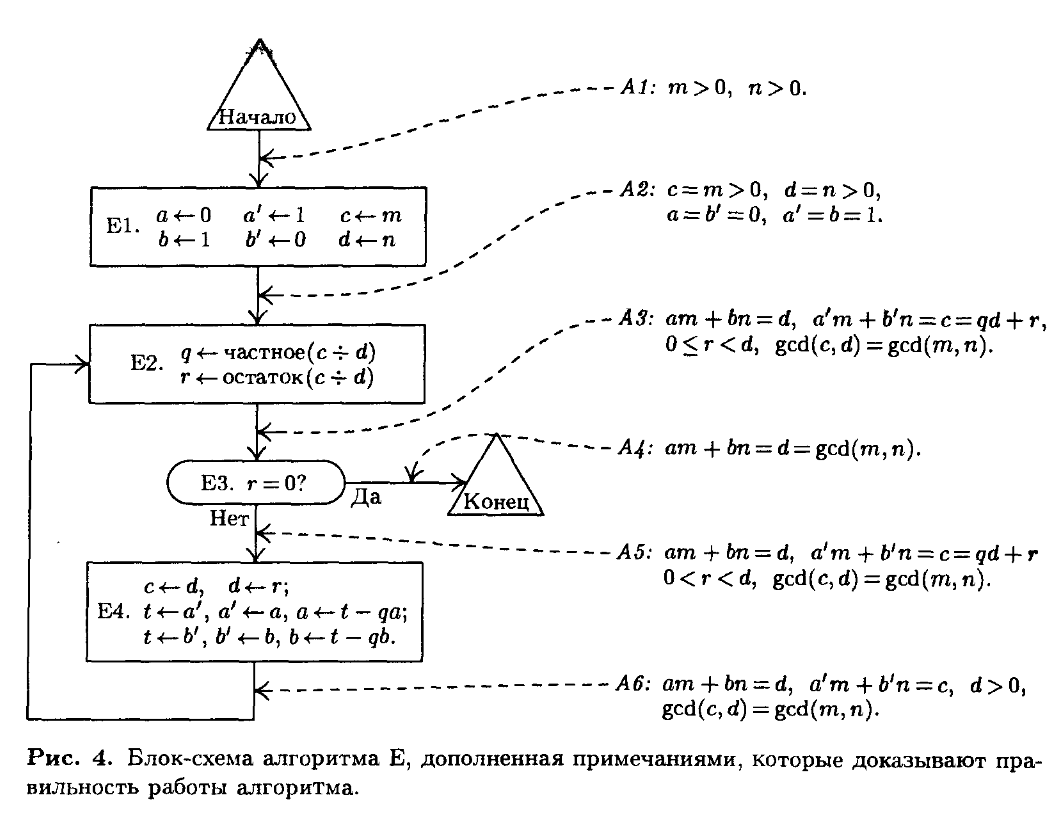
\includegraphics[scale=0.3]{ex_1_2_1_img_4_block_schema_e}

\begin{flalign*}
  & A1: T=0, m>0, n>0 & \\
  & A2: T=1, c=m>0, d=n>0, a=b'=0, a'=b=1 & \\
  & A3: T + 2 <= n - r + 2, am+bn=d, a'm+b'n=c=qd+r, 0 \leq r < d, \textrm{gcd}(c, d) = \textrm{gcd}(m,n) & \\
\end{flalign*}

Заметим, что на каждом шаге E2 выполняется условие $r<d$,следовательно $d-r \geq 1$.
Нижняя граница $n-r$ увеличивается на $1$ на каждой итерации алгоритма и достигает $n$ при $r=0$ максимум за $n$ итераций.

\begin{tabularx}{0.8\textwidth} { 
  | >{\raggedright\arraybackslash}X 
  | >{\centering\arraybackslash}X
  | >{\centering\arraybackslash}X
  | >{\centering\arraybackslash}X
  | >{\centering\arraybackslash}X | }
 \hline  $i$ & $T_6$ & $T_3$ & $T_5$ & $\inf (n-r)$ \\
 \hline  1 & --  & 2  & 3 & 1  \\
 \hline  2 & 4  & 5  & 6 & 2  \\
 \hline  3 & 7  & 8  & 9 & 3  \\
 \hline  $\cdots$ & $\cdots$  & $\cdots$  & $\cdots$ & $\cdots$  \\
 \hline  $i$ & $3i-2$  & $3i-1$  & $3i$ & $i$  \\
 \hline  $\cdots$ & $\cdots$  & $\cdots$  & $\cdots$ & $\cdots$  \\
 \hline  $last$ & $T-2$  & $T-1$  & $T \leq 3n$ & $n$  \\
 \hline
\end{tabularx}

Предположим на основании данных в таблице, что $T_5 \leq 3(n-r)$. Из этого следует, что $T_3$, $T_4$ и $T_6$ также $\leq 3(n-r)$. На основе известных утверждений об алгоритме E $r \geq 0$ на любом шаге алгоритма, следовательно $n-r \leq n$. $P(2)$, $P(3)$ следует из таблицы. Докажем по индукции $P(i+1)$.


\begin{flalign*} 
  & r_{i+1} < r_i & \\
  & T_5 \leq 3(n-r_i)& \\
  & T_{5_{i+1}} = T_{5_i} + 3 \leq 3(n-r_i)+3 = 3(n-r_i +1) \leq 3(n-r_{i+1}) & \\
  & T_{5_{i+1}} \leq 3(n-r_{i+1}) \leq 3n& \\
\end{flalign*}

\subsection{Числа, степени и логарифмы}

\subsubsection{1.}

Чему равно наименьшее положительное рациональное число?

Наименьшего положительного рационального числа не существует, т.к. для любого числа $\frac{1}{n}$ существует меньшее число $\frac{1}{n+1}$.

\subsubsection{2.}

Может ли выражение $1+0.239999999 \cdots$ быть десятичным представлением действительного числа?

Две записи в виде бесконечных десятичных дробей $1+0.23999999 \cdots$ и $1+0.2400000 \cdots$ являются представлением одного рационального числа $1 \frac{24}{100}$. По соглашениям, приведенным в данном параграфе, представление числа в виде десятичной дроби не может заканчиваться бесконечной последовательностью девяток.

\subsubsection{3.}

Чему равно $(-3)^{-3}$?

\begin{flalign*} 
  & (-3)^{-3} = -\frac{1}{27} & \\
\end{flalign*}

\subsubsection{4.}

Чему равно $(0.125)^{-\frac{2}{3}}$?

\begin{flalign*} 
  & (0.125)^{-\frac{2}{3}} = \Bigl (\frac{1}{8} \Bigl )^{-\frac{2}{3}} =
  8^{\frac{2}{3}} = (\sqrt[3]{8})^2 = 2^2 = 4 & \\
\end{flalign*}

\subsubsection{5.}

Мы определили действительные числа в терминах десятичного представления. Подумайте, как можно определить их в терминах двоичного представления, и приведите аналог соотношения (2).

\begin{flalign*} 
  & n + \frac{d_1}{2} + \frac{d_2}{4} + \cdots + \frac{d_k}{2^k}  \leq x <
  n + \frac{d_1}{2} + \frac{d_2}{4} + \cdots + \frac{d_k}{2^k} + \frac{1}{2^k} & \\
\end{flalign*}

\subsubsection{6.}

Пусть $x=m+0.d_1 d_2 \cdots$ и $y=n+0.e_1 e_2 \cdots$ --- действительные числа. Сформулируйте правило, которое на основе десятичного представления позвооляет определить, какое из неравенств верно: $x=y$, $x<y$ или $x>y$.


Если $m>n$, то $x>y$, если $m<n$, то $x<y$.
Если существует число $k$ такое, что для всех $i<k$ $d_i = e_i$, а $d_k \neq e_k$, то, при $d_k < e_k$ $x<y$, а при $d_k > e_k$ $x>y$. Если $m=n$, $d_i = e_i$ для всех $i$, то $x=y$.

\subsubsection{7.}

Для заданных чисел $x$ и $y$ докажите правила возведения в степень на основе определения (4).

\begin{flalign*} 
  & b^0 = 1, & \\
  & b^n = b^{n-1}b \textrm{, если } n>0 & \\
  & b^n = b^{n+1}/b \textrm{, если } n<0 & \\
\end{flalign*}

\begin{flalign*} 
  & b^{x+y} = b^x b^y & \\
\end{flalign*}

Для любого числа $x$ и для $y=0:$ $b^{x+0} = b^x b^0 = b^x$, т.к. $b^0=1$. Для $y=1:$ $b^{x+1} = b^x b$ согласно определению. Таким образом, $P(0)$ и $P(1)$ выполняются. Предположим по индукции, что $P(0)$, $P(1)$, $\cdots$, $P(n)$ выполняются. Тогда докажем, что выполняется и $P(n+1): b^{x+n+1} = b^x b^{n+1}$.

\begin{flalign*} 
  & b^{x+n+1} = b^{x+n} b = b^x b^n b = b^x b^{n+1} & \\
\end{flalign*}

Для $y=-1:$ $b^{x-1} = b^x/b$ согласно определению. Таким образом, $P(0)$ и $P(-1)$ выполняются. Предположим по индукции, что $P(0)$, $P(-11)$, $\cdots$, $P(-n)$ выполняются. Тогда докажем, что выполняется и $P(-n-1): b^{x-n-1} = b^x / b^{n+1}$.

\begin{flalign*} 
  & b^{x-n-1} = b^{x-n} / b = (b^x / b^n) / b = b^x / b^{n+1} & \\
\end{flalign*}


\begin{flalign*} 
  & (b^x)^y = b^{xy} & \\
\end{flalign*}

Для любого числа $x$ и для $y=0:$ $(b^x)^0 = 1 = b^0 = b^{x \cdot 0}$. Для $y=1:$ $(b^x)^1 = b^x = b^{x \cdot 1}$. Таким образом, $P(0)$ и $P(1)$ выполняются. Предположим по индукции, что $P(0)$, $P(1)$, $\cdots$, $P(n)$ выполняются. Тогда докажем, что выполняется и $P(n+1): (b^x)^{n+1} = b^{x(n+1)}$.

\begin{flalign*} 
  & (b^x)^{n+1} = (b^x)^n (b^x)^1 = b^{xn} b^x = b^{xn+x} = b^{x(n+1)} & \\
\end{flalign*}

Для $y=-1:$ $(b^x)^{-1} = 1/b^x = b^{-x} = b^{x \cdot (-1)}$. Таким образом, $P(0)$ и $P(-1)$ выполняются. Предположим по индукции, что $P(0)$, $P(-1)$, $\cdots$, $P(-n)$ выполняются. Тогда докажем, что выполняется и $P(-n-1): (b^x)^{-n-1} = b^{x(-n-1)}$.

\begin{flalign*} 
  & (b^x)^{-n-1} = (b^x)^{-n} (b^x)^{-1} = b^{-xn} b^{-x} = b^{-xn-x} = b^{x(-n-1)} & \\
\end{flalign*}

\subsubsection{8.}

Пусть $m$ -- целое положительное число. \emph{Докажите}, что у любого положительного действительного числа $u$ есть единственный положительный корень $m$-й степени, описав метод последовательного вычисления элементов десятичного представления этого корня: $n$, $d_1$, $d_2$, $\cdots$

Существует единственное целое число $n$ такое, что $ n^m \leq u < (n+1)^m $. Существует единственное целое число $0 \leq d_1 < 10$ такое, что $ (n + \frac{d_1}{10})^m \leq u < (n + \frac{d_1}{10} + \frac{1}{10})^m $. И так далее существует единственное целое число $0 \leq d_k < 10$ такое, что $ (n + \frac{d_1}{10} + \frac{d_2}{100} + \cdots + \frac{d_k}{10^k})^m \leq u <  (n + \frac{d_1}{10} + \frac{d_2}{100} + \cdots + \frac{d_k}{10^k} + \frac{1}{10^k})^m $.

\subsubsection{9.}

Для заданных рациональных чисел $x$ и $y$ докажите правила возведения в степень, предполагая, что эти правила выполняются для целых чисел $x$ и $y$.

\begin{flalign*} 
  & b^{x+y} = b^x b^y & \\
  & x = \frac{p}{q}, y = \frac{r}{s} & \\
  & b^{x+y} = b^{\frac{p}{q} + \frac{r}{s}} = b^{\frac{sp+qr}{qs}} =
  \sqrt[qs]{b^{(sp+qr)}} = \sqrt[qs]{b^{sp} b^{qr}} =
  \sqrt[qs]{b^{sp}} \sqrt[qs]{b^{qr}} = b^{\frac{sp}{qs}} b^{\frac{qr}{qs}} =
  b^{\frac{p}{q}} b^{\frac{r}{s}} = b^x b^y & \\
\end{flalign*}


Для доказательства $(b^x)^y = b^{xy}$ предварительно докажем, что $\sqrt[s]{\sqrt[q]{b}} = \sqrt[sq]{b}$. Для $s=1$ соотношение выполняется: $\sqrt[1]{\sqrt[q]{b}} = \sqrt[q]{b} = \sqrt[1 \cdot q]{b} $. Докажем, $P(n+1)$. Пусть $ v^{n+1} = v \cdot v^n = \sqrt[q]{b} $. Тогда

\begin{flalign*}
  & v = \sqrt[n+1]{\sqrt[q]{b}} & \\
  & b = (v^{n+1})^q = v^{q(n+1)} & \\
  &  v = \sqrt[q(n+1)]{b} & \\
\end{flalign*}

\begin{flalign*} 
  & (b^x)^y = b^{xy} & \\
  & x = \frac{p}{q}, y = \frac{r}{s} & \\
  & (b^x)^y = (b^{\frac{p}{q}})^{\frac{r}{s}} = \sqrt[s]{(b^{\frac{p}{q}})^r} =
  \sqrt[s]{(\sqrt[q]{b^p})^r} =
  \sqrt[s]{\underbrace{\sqrt[q]{b^p} \sqrt[q]{b^p} \cdots \sqrt[q]{b^p}}_{r \textrm{ раз}}} =
  \sqrt[s]{\sqrt[q]{\underbrace{b^p b^p \cdots b^p}_{r \textrm{ раз}}}} =
  \sqrt[s]{\sqrt[q]{(b^p)^r}} = \sqrt[s]{\sqrt[q]{b^{pr}}} =
  \sqrt[sq]{b^{pr}} = & \\
  & b^{\frac{pr}{sq}} = b^{\frac{p}{q} \frac{r}{s}} = b^{xy} & \\
\end{flalign*}

\subsubsection{10.}

Докажите, что $\log_{10}{2}$ не является рациональным числом.

Предположим, что существует число $r=\frac{p}{q}$ ($p$ -- целое, $q$ -- положительное целое) такое, что $10^r = 2$. Тогда

\begin{flalign*} 
  & 2 = 10^{\frac{p}{q}} & \\
  & 2^q = 10^p = 2^p \cdot 5^p & \\
\end{flalign*}

Таким образом, для целых $p$ и $q$ ($q>0$) имеем с одной стороны неравенства число кратное $5$, а с другой -- некратное $5$, чего быть не может.

\subsubsection{11.}

Если $b=10$ и $x \approx \log_{10}{2}$, то сколько десятичных знаков числа $x$ нужно знать, чтобы определить три первых десятичных знака в десятичном представлении $b^x$? [\emph{Замечание}. Можете использовать результаты упр. 10.]

Т.к. $\log_{10}{2}$ не является рациональным числом, то оно представимо в виде бесконечной десятичной дроби $n + \frac{d_1}{10} + \frac{d_2}{100} + \cdots + \frac{d_k}{10^k} + \cdots$ и для любого $k$ найдется число $m > k$ такое, что $d_m > 0$. При этом для любого $k$ рациональное число $10^{n + \frac{d_1}{10} + \frac{d_2}{100} + \cdots + \frac{d_k}{10^k}} < \log_{10}{2}$, а $10^{n + \frac{d_1}{10} + \frac{d_2}{100} + \cdots + \frac{d_k}{10^k} + \frac{1}{10^k}} > \log_{10}{2}$.

\subsubsection{12.}

Объясните, почему равенство $\log_{10}{2} = 0.30102999 \dots $ следует из равенств $10^{0.30102999}=1.9999999739 \dots$, $10^{0.30103000}=2.0000000199$.

Число $b$, представимое бесконечной десятичной дробью $n + \frac{d_1}{10} + \frac{d_2}{100} + \dots + \frac{d_k}{10^k} + \dots$, должно для любого $k$ удовлетворять соотношениям $n + \frac{d_1}{10} + \frac{d_2}{100} + \dots + \frac{d_k}{10^k} \leq k < n + \frac{d_1}{10} + \frac{d_2}{100} + \dots + \frac{d_k}{10^k} + \frac{1}{10^k}$.

\begin{flalign*} 
  & 1.9999999739 \leq 2 < 2.0000000199 & \\
  & 10^{0.30102999} \leq 10^{\log_{10}{2}} < 10^{0.30103000} & \\
  & 0.30102999 \leq \log_{10}{2} < 0.30103000  \textrm{ для } k=8 & \\
\end{flalign*}

Следовательно, первые 8 цифр $\log_{10}{2} = 0.30102999$.

\subsubsection{13.}

(a) Пусть $x$ --- положительное действительное число, а $n$ --- положительное целое число. Докажите неравенство $\sqrt[n]{1+x} - 1 \leq x/n$.

Для $n=1$

\begin{flalign*} 
  & 1 + x - 1 \textrm{ (?) } x & \\
  & x = x & \\
\end{flalign*}

Для $n=2$

\begin{flalign*} 
  & \sqrt{1 + x} - 1 \textrm{ (?) } x/2 & \\
  & \sqrt{1 + x} \textrm{ (?) } 1 + x/2 & \\
  & 1 + x \textrm{ (?) } (2 + x)^2/4 & \\
  & 4 + 4x \textrm{ (?) } 4 + 4x + x^2 & \\
  & 0 \leq x^2 & \\
\end{flalign*}

Предположим, что выполняются утверждения $P(0)$, $P(1)$, $\dots$, $P(n)$. Тогда для $n+1$

\begin{flalign*} 
  & \sqrt[n+1]{1+x} - 1 \textrm{ (?) } \frac{x}{n+1} & \\
  & \sqrt[n+1]{1+x} \textrm{ (?) } \frac{n+1+x}{n+1} & \\
  & 1+x \textrm{ (?) } \Bigl (1 + \frac{x}{n+1} \Bigl )^{n+1} & \\
  & 1+x \leq \Bigl (1 + \frac{x}{n} \Bigl )^{n} \textrm{ (по предположению индукции)} & \\
  & \Bigl (1+\frac{x}{n} \Bigl )^{n} \textrm{ (?) } \Bigl (1+\frac{x}{n+1} \Bigl )^{n+1} & \\
  & \Bigl (\frac{n+x}{n} \Bigl )^{n} \textrm{ (?) } \Bigl (\frac{n+1+x}{n+1} \Bigl )^{n+1} & \\
  & \frac{(n+1)^{n+1}}{n^n} \textrm{ (?) } \frac{(n+1+x)^{n+1}}{(n+x)^n} & \\
  & (n+1)\Bigl (\frac{n+1}{n} \Bigl)^n \textrm{ (?) } (n+1+x)\Bigl (\frac{n+1+x}{n+x}\Bigl )^n & \\
  & 1 \textrm{ (?) } \frac{n+1+x}{n+1} \Bigl (\frac{n}{n+1} \Bigl)^n \Bigl (\frac{n+1+x}{n+x}\Bigl )^n & \\
  & (n+1)^{n+1}(n+x)^n \textrm{ (?) } (n+1+x)^{n+1} n^n & \\
  & n^n \leq (n+1)^{n+1} & \\
  & (n+x)^n \leq (n+1+x)^{n+1} & \\
\end{flalign*}

Мы зашли в тупик. Воспользуемся подсказкой из ответов. Обозначим $y = x/n$ и докажем $\sqrt[n]{1+ny} - 1 \leq y$.

\begin{flalign*}
  & \sqrt[n]{1+ny} - 1  \textrm{ (?) } y & \\
  & 1+ny \textrm{ (?) } (1+y)^n & \\
\end{flalign*}

Данная замена оставляет в силе наши предположения по индукции. Остается доказать, что $P(n+1): 1+(n+1)y \leq (1+y)^{n+1}$.

\begin{flalign*}
  & (1+y)^{n+1} = (1+y)(1+y)^n = \underbrace{(1+y)^n + (1+y)^n \dots (1+y)^n}_{(1+y) \textrm{ раз}}  & \\
\end{flalign*}

Т.к. по предположению индукции $1+ny \leq (1+y)^n$ выполняется, то остается сравнить $y$ и $\underbrace{(1+y)^n + (1+y)^n \dots (1+y)^n}_{y \textrm{ раз}}$.

\begin{flalign*}
  & y \leq \underbrace{(1+y)^n + (1+y)^n \dots (1+y)^n}_{y \textrm{ раз}} & \\
  & 1+ny \leq (1+y)^n & \\
  & 1+(n+1)y \leq (1+y)^{n+1} & \\
\end{flalign*}

Таким образом, мы доказали, что

\begin{flalign*}
  & 1+ny \leq (1+y)^n & \\
  & 1+x \leq (1+\frac{x}{n})^n & \\
  & \sqrt[n]{1+x} \leq 1+\frac{x}{n} & \\
  & \sqrt[n]{1+x} - 1 \leq \frac{x}{n} & \\
\end{flalign*}

(b) Используйте полученный результат для доказательства утверждения.

\begin{flalign*}
  & b^{n+d_1/10 + \dots + d_k/10^k} (b^{1/10^k}-1) < b^{n+1}(b-1)/10^k & \\
\end{flalign*}

Т.к. $b>1$, то

\begin{flalign*}
  & n+d_1/10 + \dots + d_k/10^k < n+1 & \\
  & b^{n+d_1/10 + \dots + d_k/10^k} < b^{n+1} & \\
\end{flalign*}

Остается сравнить $b^{1/10^k}-1$ и $(b-1)/10^k$. Обозначим $x=b-1$, $n=10^k$ и получим уже доказанное выражение: $(x+1)^{1/n}-1 = \sqrt[n]{x+1}-1 \leq x/n$.

\subsubsection{14.}

Докажите равенство $\log_{b}{(c^y)} = y \log_{b}{c}$, если $c>0$.

Представим степень через произведение и докажем утверждение с помощью свойства логарифма произведения.
\begin{flalign*}
  & \log_{b}{(c^y)} =
  \log_{b}{(\underbrace{c \cdot c \dots c}_{y \textrm{ раз}})}  =
  \underbrace{\log_{b}{c}+\log_{b}{c}+\cdots+\log_{b}{c}}_{y \textrm{ раз}} =
  y \log_{b}{c} & \\
\end{flalign*}

Другой вариант доказательства по определению логарифма. Пусть $\log_{b}{c} = x$, тогда
\begin{flalign*}
  & b^x = c & \\
  & (b^x)^y = b^{xy} = c^y . & \\
\end{flalign*}

Отсюда $xy = \log_{b}{(c^y)} = y \log_{b}{c}$.

\subsubsection{15.}

Докажите или опровергните следующее равенство:

\begin{flalign*}
  \log_{b}{x/y}=\log_{b}{x}-\log_{b}{y} \textrm{ при } x,y > 0. \\
\end{flalign*}

Используя свойства логарифмов получаем доказательство:
\begin{flalign*}
  & \log_{b}{x/y} = \log_{b}{\Bigl (x(y)^{-1} \Bigl )} = \log_{b}{x} + \log_{b}{(y^{-1})} =\log_{b}{x}-\log_{b}{y} . & \\
\end{flalign*}

\subsubsection{16.}

Как можно выразить $\log_{10}{x}$ через $\ln{x}$ и $\ln{10}$?

\begin{flalign*}
  & \log_{10}{x} = \frac{\ln{x}}{\ln{10}}, \textrm{ так как} & \\
  & (\log_{10}{x}) (\ln{10}) =  \ln{10^{\log_{10}{x}}} = \ln{x} & \\
\end{flalign*}

\subsubsection{17.}

Чему равны $\lg{32}$, $\log_{\pi}{\pi}$, $\ln{e}$, $\log_{b}{1}$ и $\log_{b}{(-1)}$?

\begin{flalign*}
  & \lg{32}=5, \ \ \log_{\pi}{\pi}=1, \ \ \ln{e}=1, \ \ \log_{b}{1}=0, & \\
  & \log_{b}{(-1)} \textrm{ --- не существует. } & \\
\end{flalign*}

\subsubsection{18.}

Докажите или опровергните следующее равенство: $\log_{8}{x}=\frac{1}{2}\lg{x}$.

\begin{flalign*}
  & \log_{8}{x} = \frac{\lg{x}}{\lg{8}} = \frac{\lg{x}}{3} = \frac{1}{3}\lg{x}
  \neq \frac{1}{2}\lg{x} .& \\
\end{flalign*}

\subsubsection{19.}

Поместится ли целое число $n$, десятичное представление которого состоит из 14 цифр, в компьютерном слове емкостью 47 бит плюс бит знака?

Один бит может хранить $2^1=2$ числа: $0$ и $1$, в $n$ бит можно записать $2^n$ чисел от $0$ до $2^n -1$. Добавление знакового бита позволяет сохранить ещё $2^n$ чисел от $-1$ до $-2^n$.

Один десятичный разряд может представлять $10$ чисел от $0$ до $9$. С помощью $n$ десятичных разрядов можно представить $10^n$ чисел от $0$ до $10^n-1$. Таким образом, нам нужно сравнить числа $2^{47}$ и $10^{14}$.

\begin{flalign*}
  & 0.30102999 \leq \log_{10}{2} < 0.30103 & \\
  & 14 / 0.30102999 = 46.5069942034679 < 46.6 & \\
  & 14 / 0.30103 = 46.50699265853901 < 46.6 & \\
  & 10^{0.30102999} \leq 2 < 10^{0.30103} & \\
  & (10^{0.30102999})^{47} \leq 2^{47} < (10^{0.30103})^{47} & \\
  & 10^{14} < (10^{0.30102999})^{46.6} < (10^{0.30102999})^{47} \leq 2^{47} & \\
\end{flalign*}

Таким образом, для хранения числа из $14$ десятичных знаков необходимо минимум $47$ бит.


\subsubsection{20.}

Существует ли простое соотношение, связывающее $\log_{10}{2}$ и $\log_{2}{10}$?

\begin{flalign*}
  & \log_{10}{2} = \frac{\ln{2}}{\ln{10}} & \\
  & \log_{2}{10} = \frac{\ln{10}}{\ln{2}} & \\
  & \log_{10}{2} = (\log_{2}{10})^{-1} & \\
\end{flalign*}

\subsubsection{21.} (\emph{Логарифмы от логарифмов}.) Выразите $\log_{b}{\log_{b}{x}}$ через $\ln{\ln{x}}$, $\ln{\ln{b}}$ и $\ln{b}$.

\begin{flalign*}
  & \log_{b}{x} = \frac{\ln{x}}{\ln{b}} & \\
  & \log_{b}{\log_{b}{x}} = \frac{\ln{\log_{b}{x}}}{\ln{b}} =
  \frac{\ln{\frac{\ln{x}}{\ln{b}}}}{\ln{b}} =
  \frac{\ln{\ln{x}}-\ln{\ln{b}}}{\ln{b}}. & \\
\end{flalign*}

\subsubsection{22.}

(Р.В. Хемминг (R.W. Hamming).) Докажите, что

\begin{flalign*}
  \lg{x} \approx \ln{x} + \log_{10}{x}
\end{flalign*}
с погрешностью, не превышающей $1\%$! (Такми образом, таблицы натуральных и десятичных логарифмов можно использовать и для получения приближенных значений двоичных логарифмов.)

\begin{flalign*}
  & \ln{x} = \frac{\lg{x}}{\lg e} & \\
  & \log_{10}{x} = \frac{\lg{x}}{\lg {10}} & \\
  & \ln{x} + \log_{10}{x} = \frac{\lg{x}}{\lg{e}} + \frac{\lg{x}}{\lg {10}} =
  \lg {x}((\lg{e})^{-1} + (\lg{10})^{-1}) =
  \lg{x}(\ln{2} + \log_{10}{2}) & \\
  & \lg{x} = \frac{\ln{x} + \log_{10}{x}}{\ln{2} + \log_{10}{2}} & \\
  & 0.69314718 \leq \ln{2}                < 0.69314719 & \\
  & 0.30102999 \leq \log_{10}{2}          < 0.30103 & \\
  & 0.99417716 \leq \ln{2} + \log_{10}{2} < 0.99417719 . & \\
\end{flalign*}

Оценим погрешность.

\begin{flalign*}
  & \frac{\Big|\lg{x} - (\ln{x} + \log_{10}{x})\Big|}{\lg{x}} =
  \frac
      {\Big|\frac{\ln{x} + \log_{10}{x}}{\ln{2} + \log_{10}{2}} -
        (\ln{x} + \log_{10}{x})\Big|}
      {\frac{\ln{x} + \log_{10}{x}}{\ln{2} + \log_{10}{2}}} =
  \frac
      {\Big|\ln{x} + \log_{10}{x} -
        (\ln{x} + \log_{10}{x})(\ln{2} + \log_{10}{2})\Big|}
      {\ln{x} + \log_{10}{x}} = & \\
  & \frac
      {\Big|(\ln{x} + \log_{10}{x})(1-(\ln{2} + \log_{10}{2}))\Big|}
      {\ln{x} + \log_{10}{x}} = 
  \Big|(1-(\ln{2} + \log_{10}{2}))\Big| & \\
  & -0.99417719 \leq -(\ln{2} + \log_{10}{2}) < -0.99417716 & \\
  & 1-(\ln{2} + \log_{10}{2}) < 1-0.99417716 = 0.00582284 < 0.01 & \\
  & 1-(\ln{2} + \log_{10}{2}) \geq 1-0.99417719 = 0.00582281 > -0.01 & \\
  & \Big|1-(\ln{2} + \log_{10}{2})\Big| < 0.01 & \\
\end{flalign*}

\subsubsection{23.}

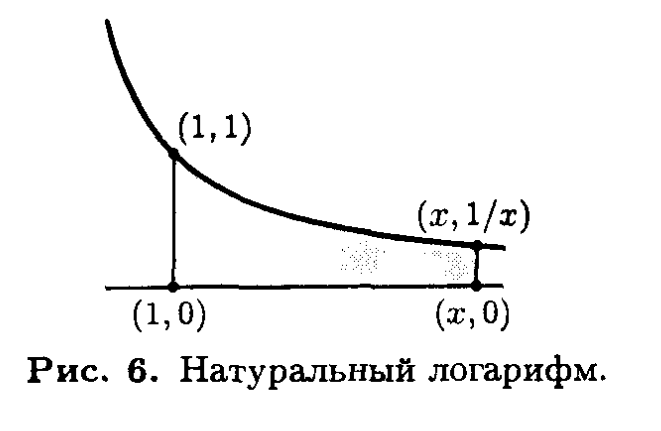
\includegraphics[scale=0.3]{ex_1_2_2_img_6_natural_log}

С помощью рис. 6 дайте \emph{геометрическое} доказательство того, что
\begin{flalign*}
  \ln{xy} = \ln{x} + \ln{y}.
\end{flalign*}

\begin{figure}[h]
  \centering
  \includegraphics[scale=0.5]{ex_1_2_2_img_6_1_Natural_log}
  \caption{Гипербола и логарифм ($x=4$, $y=25$).}
\end{figure}


Известно, что $\ln{xy}$ равен площади криволинейной трапеции под кривой $f(i) = \frac{1}{i}$ на отрезке $[1; \ xy]$, т.е. $\int\limits_1^{xy} \frac{1}{i} \ di $.

\begin{flalign*}
  & \int\limits_1^{xy} \frac{1}{i} \ di =
  \int\limits_1^{x} \frac{1}{i} \ di + \int\limits_{x}^{xy} \frac{1}{i} \ di =
  \int\limits_1^{y} \frac{1}{i} \ di + \int\limits_{y}^{xy} \frac{1}{i} \ di & \\
\end{flalign*}

Докажем, что

\begin{flalign*}
  & \int\limits_1^{x} \frac{1}{i} \ di = \int\limits_{y}^{xy} \frac{1}{i} \ di & \\
  & \int\limits_1^{y} \frac{1}{i} \ di = \int\limits_{x}^{xy} \frac{1}{i} \ di & \\
\end{flalign*}

\begin{figure}[h]
  \centering
  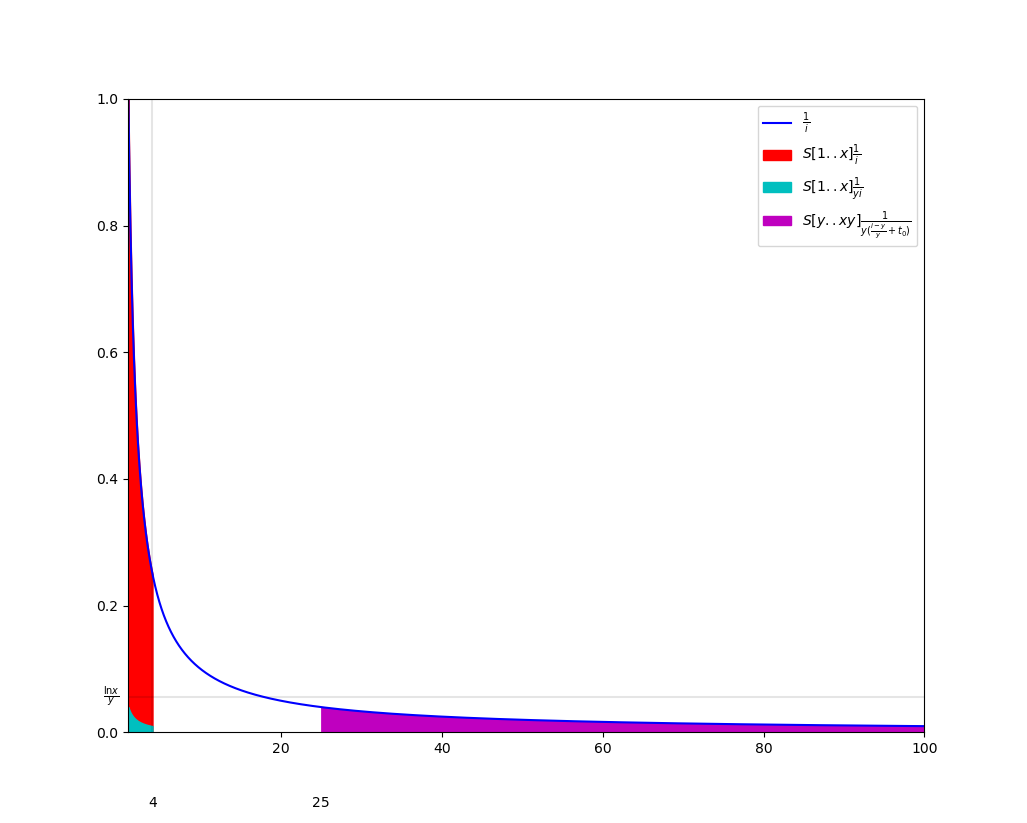
\includegraphics[width=\textwidth]{ex_1_2_2_img_6_2_log_x}
  \caption{Логарифм $x$ для $x=4$, $y=25$, $t_0=1$.}
\end{figure}

Рассмотрим $\ln{x}$. Его значение равно площади под гиперболой на отрезке $[1..x]$: $S [1..x] \frac{1}{i}$. Сожмем фигуру под гиперболой в $y$ раз относительно оси $OY$. Площадь фигуры $S [1..x] \frac{1}{y i}$ также уменьшится в $y$ раз. Затем растянем получившуюся фигуру вдоль оси $OX$ относительно вертикальной линии $y=1$ в $y$ раз (в результате площадь снова станет равной $\ln{x}$). Выполним соответствующие преобразования над кривой $\frac{1}{y i}$.

\begin{flalign*}
  & \textrm{Сначала сдвинем график влево на $1$: } && \frac{1}{y (i+1)}. & \\
  & \textrm{Длина исходной фигуры равна $x-1$.} &&& \\
  & \textrm{Длина растянутой фигуры: } && (x-1)*y & \\
\end{flalign*}

Нам нужно, чтобы значение функции равное $\ln{x}$, которое после смещения влево находится в $x-1$, переместилось в точку $y(x-1)$.

\begin{flalign*}
  & \textrm{Растянем график в $y$ раз: } && \frac{1}{y (\frac{i}{y}+1)}. & \\
  & \textrm{Сместим график вправо на $y$: } && \frac{1}{y (\frac{i-y}{y}+1)} =
  \frac{1}{i}. & \\
\end{flalign*}

Мы получили фигуру, которая лежит под кривой $\frac{1}{i}$ на отрезке $[y..xy]$. Её площадь равна $\ln{x}$. Но она же равна $\ln{xy}-\ln{y}$.

\subsubsection{24.}

Объясните, как нужно модифицировать метод вычисления логарифмов по основанию 10, приведенный в конце раздела, чтобы его можно было применить для вычисления логарифмов по основанию 2.

Предложенный метод основан на том, что
\begin{flalign*}
  & 1 \leq x_k = x^{2^k}/10^{2^k(n+b_1/2+\dots+b_k/2^k)} < 10 & \\
  & 10^{2^k(n+b_1/2+\dots+b_k/2^k)} \leq x^{2^k} <
    10^{2^k(n+b_1/2+\dots+b_k/2^k)+1} & \\
  & 10^{n+b_1/2+\dots+b_k/2^k} \leq x < 10^{n+b_1/2+\dots+b_k/2^k+1/2^k} & \\
\end{flalign*}

Действительно:
\begin{flalign*}
  & x_0 = \Bigl(\frac{x}{10^n}\Bigl); & \\
  & x_1 = \Bigl(\frac{x}{10^n}\Bigl)^2*\frac{1}{10^{b_1}} =
  \Bigl(\frac{x}{10^n}\Bigl)^2*\Bigl(\frac{1}{10^{\frac{b_1}{2}}}\Bigl)^2 =
  \frac{x^{2^1}}{10^{2^1(n+\frac{b_1}{2})}} & \\
  & x_2=\Bigl(\frac{x^{2}}{10^{2(n+\frac{b_1}{2})}}\Bigl)^2*\frac{1}{10^{b_2}} =
  \Bigl(\frac{x^{2}}{10^{2(n+\frac{b_1}{2})}}\Bigl)^2*
    \Bigl(\frac{1}{10^{\frac{b_2}{4}}}\Bigl)^4 =
    \frac{x^{2^2}}{10^{2^2(n+\frac{b_1}{2}+\frac{b_2}{4})}} & \\
  & \cdots & \\
  & x_k=\frac{x^{2^k}}{10^{2^k(n+b_1/2+\dots+b_k/2^k)}}  & \\
  & (x^{2^k})^2 = x^{2^k \cdot 2^1} = x^{2^{k+1}} & \\  
  & x_{k+1}=\Bigl(\frac{x^{2^k}}{10^{2^k(n+b_1/2+\dots+b_k/2^k)}}\Bigl)^2*
    \Bigl(\frac{1}{10^{\frac{b_{k+1}}{2^{k+1}}}}\Bigl)^{2^{k+1}} =
  \frac{x^{2^{k+1}}}{10^{2^{k+1}(n+b_1/2+\dots+b_k/2^k + b_{k+1}/2^{k+1})}} & \\  
\end{flalign*}

Модифицируем предложенный метод в соответствии с заданием.
\begin{flalign*}
  & 2^{n+b_1/2+\dots+b_k/2^k} \leq x < 2^{n+b_1/2+\dots+b_k/2^k+1/2^k} & \\
  & 2^{2^k(n+b_1/2+\dots+b_k/2^k)} \leq x^{2^k} <
    2^{2^k(n+b_1/2+\dots+b_k/2^k)+1} & \\
  & 1 \leq x_k = x^{2^k}/2^{2^k(n+b_1/2+\dots+b_k/2^k)} < 2 & \\
\end{flalign*}

Сначала сдвинем десятичную точку в числе $x$ влево или вправо, чтобы получить $1 \leq x/2^n < 2$; таким образом мы определим целую часть числа $\lg{x}$, т.е. $n$. Чтобы найти значения $b_1$, $b_2$, $\cdots$, положим $x_0=x/10^n$ и для $k \geq 1$ получим
\begin{flalign*}
  & b_k = 0, & x_k=x_{k-1}^2, && \textrm{если} && x_{k-1}^2 < 2; && \\
  & b_k = 1, & x_k=x_{k-1}^2/2, && \textrm{если} && x_{k-1}^2 \geq 2. && \\
\end{flalign*}

\subsubsection{25.}
Предположим, что у нас есть двоичный компьтер (т.е. компьютер, в котором используется двоичная система счисления. --- \textit{Прим. перев.}) и имеется некоторое число $x$, $1 \leq x < 2$. Покажите, что следующий алгоритм, в котором используются только операции сдвига, сложения и вычитания в объеме, пропорциональном числу разрядов, которое определяется требуемой степенью точности, можно применить для приближенного вычисления $y=\log_{b}{x}$.

\textbf{L1.} [Инициализация.] Присвоить $y \leftarrow 0$, $z \leftarrow x$ с помощью сдвига вправо на $1$, $k \leftarrow 1$.

\textbf{L2.} [Проверка окончания.] Если $x=1$, то прекратиь выполнение.

\textbf{L3.} [Сравнение.] Если $x-z<1$, то присвоить $z \leftarrow z$ с помощью сдвига вправо на $1$, $k \leftarrow k+1$, и повторить этот шаг.

\textbf{L4.} [Замещение значений.] Присвоить $x \leftarrow x-z$, $z \leftarrow x$ с помощью сдвига вправо на $k$, $y \leftarrow y+\log_{b}{2^k/(2^k-1)}$ и перейти к шагу L2. $\bigl \bracevert$

[\textit{Замечание.} Описанный метод очень похож на тот метод, который используется в компьютерах для выполнения операции деления. Эта идея, в сущности, принадлежит Генри Бриггсу (Henry Briggs); он применял данный метод (только не к двоичным, а к десятичным операциям) для вычисления таблиц логарифмов, опубликованных в 1624 году. Нам нужна дополнительная таблица констант $\log_b{2}$, $\log_b{(4/3)}$, $\log_b{(8/7)}$ и т.д. до значения, равного точности компьютера. В данном алгоритме преднамеренно делается ошибка, так как числа сдвигаются вправо с тем, чтобы в конечном счете $x$ свелось к $1$ и выполнение алгоритма прекратилось. В этом упражнении вы должны показать, что алгоритм конечен и вычисляет приближенное значение $\log_b{x}$.]

Рассмотрим условия, которые выполняются в процессе рабоы алгоритма.

A1. $1 \leq x < 2$, $y=0$, $0<z<1$, $k=1$, $z<x$, $\frac{x}{z}=2$.

A2.

A3. $0 \leq z < 1$, $k \geq 1$, $x-z \geq 1$, $z<x$.

A4. $1 \leq x<2$, $0 \leq z<1$, $k \geq 1$, $2^k \geq 2$, $1<\frac{2^k}{2^k-1} \leq 2$, $z<x$.

Доказать применимость алгоритма для вычисления приближенных значений $\log_{b}{x}$ можно, сравнив значения переменной $y$ на каждой итерации алгоритма с точным значением $\log_{b}{x}$.

\begin{flalign*}
  & y = \log_b{\frac{2^{k_1}}{2^{k_1}-1}} + \log_b{\frac{2^{k_2}}{2^{k_2}-1}} +
  \cdots + \log_b{\frac{2^{k_n}}{2^{k_n}-1}}.& \\
\end{flalign*}

Рассмотрим свойства последовательности $k_1$, $k_2$, $\cdots$, $k_n$.

В результате выполнения алгоритма число $x$ последовательно уменьшается на величину $z$:

\begin{flalign*}
  & x_1 = x - \frac{x}{2^{k_1}} = x(1 - \frac{1}{2^{k_1}}) = x \frac{2^{k_1}-1}{2^{k_1}}; & \\
  & x_2 = x_1(1 - \frac{1}{2^{k_2}}) = x_1 \frac{2^{k_2}-1}{2^{k_2}}; & \\
  & \cdots & \\
  & x_n = x_{n-1} \frac{2^{k_n}-1}{2^{k_n}} \approx 1. & \\
\end{flalign*}

Таким образом $x$ приближенно можно представить в виде дроби:
\begin{flalign} \label{eq:1_2_2__25_1}
  & x = \frac{2^{k_1}}{2^{k_1}-1} x_1 =
  \frac{2^{k_1} 2^{k_2}}{(2^{k_1}-1)(2^{k_2}-1)} x_2 =
  \cdots \approx
  \frac{2^{k_1} 2^{k_2}\cdots 2^{k_n}}{(2^{k_1}-1)(2^{k_2}-1)\cdots(2^{k_n}-1)}.&
\end{flalign}

Соответственно:
\begin{flalign*}
  & y = \log_b{x} \approx \log_b{
    \frac{2^{k_1}2^{k_2}\cdots 2^{k_n}}{(2^{k_1}-1)(2^{k_2}-1)\cdots(2^{k_n}-1)}}=
  \log_b{\frac{2^{k_1}}{2^{k_1}-1}} + \log_b{\frac{2^{k_2}}{2^{k_2}-1}} +
  \cdots + \log_b{\frac{2^{k_n}}{2^{k_n}-1}}.& \\
\end{flalign*}

Докажем конечность алгоритма. Считаем, что алгоритм будет выполняться бесконечно тогда и только тогда, когда на одной из итераций перед шагом \textbf{L4} $x>1$, а $z=0$.

На всех шагах алгоритма кроме последнего $x>1$. Если $x>1$, то такое число представляется в виде единицы перед запятой и некоторого количества единиц после. При сдвиге вправо на $k$ разрядов единица перед запятой будет сдвигаться вправо. При этом важно, чтобы $k$ не превышало числа разрядов после запятой до тех пор, пока число $x>1$. Это так, потому что $k$ последовательно увеличивается на $1$ только в том случае, если $z$ настолько велико, чтобы сделать $x < 1$. А в этом случае $z$ содержит хотя бы одну единицу не в последнем разряде, соответственно $k$ меньше числа разрядов.  Поэтому всегда найдется такое $z$, получаемое в результате сдвига числа $x$ на $k$ разрядов вправо, что либо $x-z < x$ и $z>0$, либо $x=1$.

\subsubsection{26.}

Определите верхние границы точности алгоритма из предыдущего упражнения, взяв за основу точность, используемую в арифметических операциях.

Предыдущий алгоритм вычисляет логарифмы с определенной погрешностью $\delta$. Истинное значение логарифма лежит в интервале $[y-\delta; y+\delta]$. Точностью алгоритма можно считать разность между верхней и нижней границами данного интервала $2\delta$. Требуется определить каким образом точность ограничена сверзху.

Пусть $p$ -- количество разрядов после двоичной точки. После выполнения шага \textbf{L4} $z=\frac{x_i}{2^k}$. Если $z=0$, то $k=p+1$, т.к. $x \geq 1$ и чтобы обнулить его сдвигом вправо нужно сдвинуть единицу в целой части на $k+1$ разрядов. Как уже показано, такого не может быть, т.е. $z>0$.

Действительное число $x$ может быть представлено в компьютере в виде числа в двоичной системе счисления с фиксированным количеством разрядов после запятой. В формуле \ref{eq:1_2_2__25_1} для представления $x$ используется деление на 2, а в алгоритме -- сдвиг вправо на 1. Сдвиг отличается от деления, например в двоичной системе счисления и четырьмя разрядами после точки $10.0001>>1=1.0000$, хотя истинное значение $10.0001/2=1.00001$. Таким образом, на каждой итерации значения $z$ и $x$ вычисляются с точностью $\frac{1}{2^p}$. Количество итераций не может превышать $p$, следовательно общая погрешность вычислений должна быть меньше $\frac{p}{2^p}$. С другой стороны мы ограничены точностью компьютера $\frac{1}{2^p}$.

\subsubsection{27.}

Рассмотрим метод вычисления $\log_{10}{x}$, описанный в этом разделе. Пусть $x_k'$ --- вычисленное приближенное значение $x_k$, причем $x_0$ определяется из соотношения $x(1-\delta) \leq 10^n x_0' \leq x(1+\epsilon)$, а $x_k'$ --- из соотношений
\begin{flalign*}
  & b_k = 0, & x_k=x_{k-1}^2, && \textrm{если} && x_{k-1}^2 < 10; && \\
  & b_k = 1, & x_k=x_{k-1}^2/10, && \textrm{если} && x_{k-1}^2 \geq 10, && \\
\end{flalign*}
где выражение $(x_{k-1}')^2$ нужно заменить на $y_k$ и $(x_{k-1}')^2(1-\delta) \leq y_k \leq (x_{k-1}')^2(1+\epsilon)$, где $1\leq y_k < 100$. В этих формулах $\delta$ и $\epsilon$ --- малые константы, соответствующие верхней и нижней границам погрешностей округления. Покажите, что если результат вычислений обозначить $\log'{x}$, то через $k$ шагов мы получим
\begin{flalign*}
  & \log_{10}{x} + 2 \log_{10}{(1-\delta)} - 1/2^{k} < \log'{x} \leq
  \log_{10}{x} + 2\log_{10}(1+\epsilon). & \\
\end{flalign*}

Данный метод вычислений логарифмов основан на том, что
\begin{flalign*}
  & 10^{n+b_1/2+b_2/4+\cdots+b_k/{2^k}} \leq x=10^y < 10^{n+b_1/2+b_2/4+\cdots+b_k/{2^k}+1/{2^k}}; & \\
  & 10^{2^k(n+b_1/2+b_2/4+\cdots+b_k/{2^k})} \leq x^{2^k} < 10^{2^k(n+b_1/2+b_2/4+\cdots+b_k/{2^k})+1}; & \\
  & 1 \leq x^{2^k}/10^{2^k(n+b_1/2+b_2/4+\cdots+b_k/{2^k})} < 10. & \\
\end{flalign*}

За $y$ мы обозначили точное значение $\log_{10}{x}$, а за $\log'{x}=n+b_1/2+b_2/4+\cdots+b_k/{2^k}$ приближенное значение. Тогда
\begin{flalign*}
  & \log'{x} \leq \log_{10}{x} < \log'{x}+1/2^k & \\
  & 0 \leq \log_{10}{x} -\log'{x} < 1/2^k & \\
  & -1/2^k < \log'{x} -\log_{10}{x} \leq 0  & \\
\end{flalign*}
\begin{flalign} \label{eq:1_2_2__27_1}
  & \log_{10}{x}-1/2^k < \log'{x} \leq \log_{10}{x}  &
\end{flalign}

Теперь введем в рассмотрение погрешность вычислений.
\begin{flalign*}
  & \Bigl(\frac{x(1-\delta)}{10^n}\Bigl) \leq x_0 \leq \Bigl(\frac{x(1+\epsilon)}{10^n}\Bigl); & \\
  & (x_0)^2*\frac{(1-\delta)}{10^{b_1}} = \frac{x^{2^1} (1-\delta)^3}{10^{2^1(n+\frac{b_1}{2})}} \leq
  x_1 \leq (x_0)^2*\frac{(1+\epsilon)}{10^{b_1}}=\frac{x^{2^1} (1+\epsilon)^3}{10^{2^1(n+\frac{b_1}{2})}} &\\
  & \frac{x^{2^2}(1-\delta)^7}{10^{2^2(n+\frac{b_1}{2}+\frac{b_2}{4})}} \leq x_2
  \leq \frac{x^{2^2}(1+\epsilon)^7}{10^{2^2(n+\frac{b_1}{2}+\frac{b_2}{4})}} & \\
  & \cdots & \\
\end{flalign*}
\begin{flalign*}
  & k: && 0,&& 1,&& 2,&& 3,&& 4,&& \dots  & \\
  & n=2(n-1)+1: && 1,&& 3,&& 7,&& 15,&& 31,&& \dots  & \\
  & n=2(n-1): && 0,&& 2,&& 6,&& 14,&& 30,&& \dots  & \\
  & n=2^k: && 1,&& 2,&& 4,&& 8,&& 16,&& \dots & \\
  & n=2^{k+1}-1: && 1,&& 3,&& 7,&& 15,&& 31,&& \dots & \\
\end{flalign*}
\begin{flalign*}
  & 1 \leq \frac{x^{2^k}(1-\delta)^{2^{k+1}-1}}{10^{2^k(n+b_1/2+\dots+b_k/2^k)}}
  \leq x_k \leq
  \frac{x^{2^k}(1+\epsilon)^{2^{k+1}-1}}{10^{2^k(n+b_1/2+\dots+b_k/2^k)}}= & \\
  & \frac{x^{2^k}\Bigl((1+\epsilon)^2\Bigl)^{2^k}}{10^{2^k(n+b_1/2+\dots+b_k/2^k)}(1+\epsilon)} \leq
  \frac{x^{2^k}\Bigl((1+\epsilon)^2\Bigl)^{2^k}}{10^{2^k(n+b_1/2+\dots+b_k/2^k)}}
  <10& \\
\end{flalign*}

Таким образом вместо $\log_{10}{x}$ получаем выражения $\log_{10}{x(1-\delta)^2}$ и $\log_{10}{x(1+\epsilon)^2}$ соответственно, которые нужно подставить в \ref{eq:1_2_2__27_1}.

\subsubsection{28.}

(Р. Фейман (R. Feynman).) Придумайте метод вычисления $b^x$, где $0 \leq x < 1$, используя только операции сдвига, сложения и вычитания (аналогично алгоритму из упр. 25), и проанализируйте его точность.

В упражнении 25 мы получили приближенное значение логарифма

\begin{flalign*}
  & x = \log_b{\frac{2^{k_1}}{2^{k_1}-1}} + \log_b{\frac{2^{k_2}}{2^{k_2}-1}} +
  \cdots + \log_b{\frac{2^{k_n}}{2^{k_n}-1}};& \\
  & y = b^x \approx
  \frac{2^{k_1} 2^{k_2}\cdots 2^{k_n}}{(2^{k_1}-1)(2^{k_2}-1)\cdots(2^{k_n}-1)}.&
\end{flalign*}

Таким образом, базовая идея состоит в том, чтобы при наличии таблицы логарифмов последовательно уменьшать $x$ на величину $\log_{b}{\frac{2^{k_i}}{2^{k_i}-1}}$ до тех пор, пока он не станет равным $0$. Одновременно с этим умножать $y$ на $\frac{2^{k_i}}{2^{k_i}-1}$. Проблема заключается в том, чтобы вычислить $y$, не прибегая к умножению:
\begin{flalign*}
  & y_1 = 1 \frac{2^{k_1}}{2^{k_1}-1}; & \\
  & \frac{1}{y_1} = \frac{2^{k_1}-1}{2^{k_1}} = 1 - \frac{1}{2^{k_1}}. & \\
\end{flalign*}

В ответе к упражнению в качестве начального значения $y$ берется не $1$, а некоторое приближенное значение $b^{(1-\epsilon)}$, где $1-\epsilon \approx x$. Тогда алгоритм состоит в последовательном вычитании из $y_{i-1}$ $\frac{y_{i-1}}{2^{k_i}}$, как в упражнении 25. Как вычислить приближенное значение $b^{(1-\epsilon)}$ в ответах умалчивается.

\subsubsection{29.}
Пусть $x$ --- действительное число, большее, чем $1$. (a) При каком действительном $b > 1$ величина $b \log_{b}{x}$ минимальна? (b) При каком \emph{целом} $b>1$ эта величина минимальна? (c) При каком целом $b>1$ величина $(b+1)\log_{b}{x}$ минимальна?

(a) Функция $\log_{b}{x}$ является монотонно возрастающей. Чем больше значение $b$, тем меньше значение функции. С другой стороны, чем больше $b$, тем больше значение функции $b \cdot t$. Зафиксируем $x=t_0 > 1$ и рассмотрим функцию $f(b) = b \log_{b}{t_0}$.
\begin{flalign*}
  & (b \log_{b}{t_0})' = b'\log_{b}{t_0} + b (\log_{b}{t_0})' = 
  \log_{b}{t_0} + b\Bigl(\frac{\ln{t_0}}{\ln{b}} \Bigl)' =
  \log_{b}{t_0} -\frac{b\ln{t_0}}{(\ln{b})^2} (\ln{b})' = \log_{b}{t_0} -\frac{b\ln{t_0}}{b(\ln{b})^2} = & \\
  & \frac{\ln{t_0}}{\ln{b}} - \frac{\ln{t_0}}{(\ln{b})^2} =
  \ln{t_0}\frac{\ln{b}-1}{(\ln{b})^2} & \\
  & (b \log_{b}{t_0})' =  \Bigl( \frac{b \ln{t_0}}{\ln{b}}\Bigl)'=
  \frac{\ln{t_0}\ln{b} - \frac{b\ln{t_0}}{b}}{(\ln{b})^2} =
  \ln{t_0}\frac{\ln{b}-1}{(\ln{b})^2}& \\
\end{flalign*}

Производная функции равна $0$, когда $b=e$.

(b) Так как в точке $e$ функция $f(b) = b \log_{b}{t_0}$ имеет локальный экстремум, то при $b < e$ функция убывает, а при $b > e$ -- возрастает. Следовательно при $b = 2$ и $b = 3$ функция ближе всего к своему минимальному значению.
\begin{flalign*}
  & 2 \log_{2}{x} \textrm{ (?) } 3 \log_{3}{x} & \\
  & 2 \frac{\log_{3}{x}}{\log_{3}{2}} \textrm{ (?) } 3 \log_{3}{x} & \\
  & \frac{2}{3} \textrm{ (?) } \log_{3}{2} & \\
  & 0.666 > 0.630 & \\
  & 2 \log_{2}{x} > 3 \log_{3}{x} & \\
\end{flalign*}

Таким образом, при $b=3$ функция минимальна.

(c) Найдем производную функции $f(b) = (b+1) \log_{b}{t_0}$.
\begin{flalign*}
  & ((b+1) \log_{b}{t_0})' =  \ln{t_0} \Bigl( \frac{(b+1)}{\ln{b}}\Bigl)'=
  \ln{t_0} \frac{\ln{b} - \frac{b+1}{b}}{(\ln{b})^2} =
  \ln{t_0}\frac{\ln{b}-1-\frac{1}{b}}{(\ln{b})^2}& \\
  & \ln{b} = 1+\frac{1}{b} & \\
  & e^{\ln{b}} = e^{1+\frac{1}{b}} & \\
  & b = e \sqrt[b]{e} & \\
  & b^b = e^b e & \\
  & \Bigl(\frac{b}{e}\Bigl)^b = e & \\
  & t = \frac{b}{e} & \\
  & t^{et} = e& \\
  & t^t = e^{\frac{1}{e}}& \\
\end{flalign*}

Выразить $t$ простым способом не получилось.

Сравним последовательно функцию $f(b)$ при разных значениях $b$.

\begin{flalign*}
  & 3 \log_{2}{x} \textrm{ (?) } 4 \log_{3}{x} & \\
  & \frac{3}{4} \textrm{ (?) } \log_{3}{2} & \\
  & 0.75 > 0.63 & \\
  & 3 \log_{2}{x} > 4 \log_{3}{x} & \\
\end{flalign*}

На отрезке $2 \leq b \leq 3$ функция убывает. Сравниваем дальше.
\begin{flalign*}
  & 4 \log_{3}{x} \textrm{ (?) } 5 \log_{4}{x} & \\
  & \frac{4}{5} \textrm{ (?) } \log_{4}{3} & \\
  & 0.8 > 0.792 & \\
  & 4 \log_{3}{x} > 5 \log_{4}{x} & \\
\end{flalign*}

\begin{flalign*}
  & 5 \log_{4}{x} \textrm{ (?) } 6 \log_{5}{x} & \\
  & \frac{5}{6} \textrm{ (?) } \log_{5}{4} & \\
  & 0.833 < 0.861 & \\
  & 5 \log_{4}{x} < 6 \log_{5}{x} & \\
\end{flalign*}

Таким образом, при $b=4$ функция минимальна.

\subsection{Суммы и произведения}

\subsubsection{1.}

Что означает запись $\sum_{1 \leq j \leq n}{a_j}$ для $n=3.14$?
\begin{flalign*}
  & \sum_{1 \leq j \leq 3.14}{a_j} = a_1 + a_2 + a_3. & \\
\end{flalign*}

\subsubsection{2.}

Не пользуясь знаком $\sum$, запишите эквивалент выражения
\begin{flalign*}
  & \sum_{0 \leq n \leq 5}{\frac{1}{2n+1}}, & \\
\end{flalign*}
а также выражения
\begin{flalign*}
  & \sum_{0 \leq n^2 \leq 5}{\frac{1}{2n^2+1}}. & \\
\end{flalign*}

\begin{flalign*}
  & \sum_{0 \leq n \leq 5}{\frac{1}{2n+1}} = \frac{1}{1} + \frac{1}{3} + \frac{1}{5} + \frac{1}{7} + \frac{1}{9} + \frac{1}{11} = 1 + \frac{4}{9} + \frac{12}{35}+\frac{1}{11} = 1 + \frac{4}{9} + \frac{167}{385} = 1 \frac{3043}{3465}; & \\
  & \sum_{0 \leq n^2 \leq 5}{\frac{1}{2n^2+1}} = \sum_{-\sqrt{5} \leq n \leq \sqrt{5}}{\frac{1}{2n^2+1}} = \frac{1}{2(-2)^2+1}+\frac{1}{2(-1)^2+1}+\frac{1}{2(0)^2+1}+\frac{1}{2(1)^2+1}+\frac{1}{2(2)^2+1} = \frac{2}{9} + \frac{2}{3} + \frac{1}{1}. & \\
\end{flalign*}

\subsubsection{3.}

Объясните, почему несмотря на правило (b) результаты предыдущего упражнения различны.

Стоит отметить, что $\sum_{0 \leq n^2 \leq 5}{\frac{1}{2n^2+1}} \neq \sum_{0 \leq i \leq 5}{\frac{1}{2i+1}}$, т.к. $i = p(n)=n^2$ ($ n=\pm \sqrt{i} $) не является перестановкой в области суммирования.
\begin{flalign*}
  & R(p(n)) = [0 \leq n^2 \leq 5]; & \\
  & R(i) = [0 \leq i \leq 5]; & \\
  & i=0: \ \ \sum_{n}{[i=p(n)]} = \sum_{n=0}{[i=p(n)]} = 1; & \\
  & i=1: \ \ \sum_{n}{[i=p(n)]} = \sum_{n=\pm 1}{[i=p(n)]} = 2; & \\
  & i \in \{2,3,5\}: \ \ \sum_{n}{[i=p(n)]} = 0; & \\
  & i=4: \ \ \sum_{n}{[i=p(n)]} = \sum_{n=\pm 2}{[i=p(n)]} = 2; & \\
  & \sum_{0 \leq n^2 \leq 5}{\frac{1}{2n^2+1}} = \sum_{0 \leq i \leq 5}{\frac{1}{2i+1} \sum_{n}{[i=p(m)]}} = \frac{1}{2 \cdot 0+1}+\frac{2}{2 \cdot 1+1}+\frac{2}{2 \cdot 4+1} = \frac{2}{9} + \frac{2}{3} + \frac{1}{1}. & \\
\end{flalign*}

\subsubsection{4.}

Не пользуясь знаком ``$\sum$'', запишите эквиваленты каждой части равенства (10) как суммы сумм для случая $n=3$.
\begin{flalign*}
  & \sum_{i=1}^{3}{\sum_{j=1}^{i}{a_{ij}}} = \sum_{j=1}^{3}{\sum_{i=j}^{3}{a_{ij}}}; & \\
  & \sum_{i=1}^{3}{\sum_{j=1}^{i}{a_{ij}}} = \sum_{j=1}^{1}{a_{1j}} + \sum_{j=1}^{2}{a_{2j}} + \sum_{j=1}^{3}{a_{3j}} = (a_{11}) + (a_{21}+a_{22}) + (a_{31}+a_{32}+a_{33}); & \\
  & \sum_{j=1}^{3}{\sum_{i=j}^{3}{a_{ij}}} = \sum_{i=1}^{3}{a_{i1}} + \sum_{i=2}^{3}{a_{i2}} + \sum_{i=3}^{3}{a_{i3}} = (a_{11}+a_{21}+a_{31})+(a_{22}+a_{32})+(a_{33}); & \\
\end{flalign*}

\subsubsection{5.}

Докажите, что правило (a) справедливо для произвольного бесконечного ряда при условии, что этот ряд сходится.
\begin{flalign*}
  & \Bigl(\sum_{R(i)}{a_i}\Bigl)\Bigl(\sum_{S(j)}{b_j}\Bigl) = \sum_{R(i)}{\sum_{S(j)}{a_i b_j}}. & \\
\end{flalign*}
Если бесконечный ряд $a_i$ сходится, то
\begin{flalign*}
  & \sum_{i \geq 0}{a_i} = \lim_{n \rightarrow \infty}{\sum_{0 \leq i < n}{a_i}} = S_a & \\
\end{flalign*}
и данный предел существует. Аналогично для ряда $b_j$ существует предел
\begin{flalign*}
  & \sum_{j \geq 0}{b_j} = \lim_{n \rightarrow \infty}{\sum_{0 \leq j < n}{b_j}} = S_b. & \\
\end{flalign*}
Тогда
\begin{flalign*}
  & \Bigl(\sum_{R(i)}{a_i}\Bigl)\Bigl(\sum_{S(j)}{b_j}\Bigl)=S_a \cdot S_b=
  \lim_{n \rightarrow \infty}{\sum_{0 \leq i < n}{a_i}} \cdot \lim_{n \rightarrow \infty}{\sum_{0 \leq j < n}{b_j}} =
  \lim_{n \rightarrow \infty}{\Bigl(\sum_{0 \leq i < n}{a_i}\Bigl)\Bigl( \sum_{0 \leq j < n}{b_j}\Bigl)} =
  \lim_{n \rightarrow \infty}{\sum_{0 \leq i < n}\Bigl({a_i} \sum_{0 \leq j < n}{b_j}\Bigl)} = & \\
 & \lim_{n \rightarrow \infty}{\sum_{0 \leq i < n}{\sum_{0 \leq j < n}{a_i b_j}}}.& \\
\end{flalign*}

\subsubsection{6.}

Докажите, что правило (d) справедливо для произвольного бесконечного ряда при условии, что сходятся любые три суммы из четырех.
\begin{flalign*}
  & \sum_{R(j)}{a_j} + \sum_{S(j)}{a_j} = \sum_{R(j) \textrm{ или } S(j)}{a_j} + \sum_{R(j) \textrm{ и } S(j)}{a_j}; & \\
  & \lim{\sum_{R(j)}{a_j}} + \lim{\sum_{S(j)}{a_j}} = \lim{\Bigl(\sum_{R(j)}{a_j} + \sum_{S(j)}{a_j}\Bigl)}. & \\
\end{flalign*}
Возьмем один элемент $a_{j_1}$ из второй суммы, который не встречается в первой сумме, и перенесем его в первую сумму: 
\begin{flalign*}
  & \lim{\Bigl(\sum_{R(j) \textrm{ или } j \in \{j_1\}}{a_j} + \sum_{S(j) \textrm{ и } j \notin \{j_1\}}{a_j} \Bigl)}. & \\
\end{flalign*}
Продолжим переносить таким образом элементы до тех пор, пока во второй сумме останутся только те элементы, которые есть и в первой сумме:
\begin{flalign*}
  & \lim{\Bigl(\sum_{R(j) \textrm{ или } j \in \{j_1, j_2\}}{a_j} + \sum_{S(j) \textrm{ и } j \notin \{j_1, j_2\}}{a_j} \Bigl)}; & \\
  & \cdots & \\
  & \lim{\Bigl(\sum_{R(j) \textrm{ или } j \in \{j_1, j_2, \dots, j_k\}}{a_j} + \sum_{S(j) \textrm{ и } j \notin \{j_1, j_2, \dots, j_k\}}{a_j} \Bigl)}. & \\
\end{flalign*}

Утверждение $[R(j) \textrm{ или } j \in \{j_1, j_2, \dots, j_k\}]$ эквивалентно $[R(j) \textrm{ или } S(j)]$ т.к. все остальные элементы $j_{k+1}, j_{k+2}, \dots$ в $S(j)$ уже входят в $R(j)$. А утверждение $[S(j) \textrm{ и } j \notin \{j_1, j_2, \dots, j_k\}]$ эквивалентно $[R(j) \textrm{ и } S(j) ]$, т.к. все элементы $j_{k+1}, j_{k+2}, \dots$ входят и в $R(j)$, и в $S(j)$. Таким образом, мы получаем
\begin{flalign*}
  & \lim{\Bigl(\sum_{R(j)\textrm{ или }S(j)}{a_j}+\sum_{S(j)\textrm{ и }R(j)}{a_j} \Bigl)} = \lim{\sum_{R(j)\textrm{ или }S(j)}{a_j}}+\lim{\sum_{S(j)\textrm{ и }R(j)}{a_j}}. & \\
\end{flalign*}

\subsubsection{7.}
Покажите, что если $c$ --- любое целое число, то $\sum_{R(j)}{a_j}=\sum_{R(c-j)}{a_{c-j}}$, даже если оба ряда бесконечны.

Пусть $i = p(j) = c-j$. При этом каждому значению $j$ соответствует одно и только одно значение $i$. Тогда для бесконечного ряда $a_{p(j)}$
\begin{flalign*}
  & \lim_{n \rightarrow \infty} {\sum_{\substack{R(p(j))\\-n<j<n}}{a_{p(j)}}} =
  \sum_{i}{a_i [R(i)] \sum_{j}{[i=p(j)=c-j]}} =
  \sum_{i}{a_i [R(i)]} = \sum_{j}{a_j [R(j)]} =
  & \lim_{n \rightarrow \infty} {\sum_{\substack{R(j)\\-n<j<n}}{a_{j}}}. & \\
\end{flalign*}

\subsubsection{8.}
Приведите пример бесконечного ряда, для которого равенство (7) ложно.
\begin{flalign*}
  & \sum_{R(i)}{\sum_{S(j)}{a_{ij}}} = \sum_{S(j)}{\sum_{R(i)}{a_{ij}}}. & \\
\end{flalign*}

Утверждается, что равенство (7) справедливо для абсолютно сходящихся бесконечных рядов.
Возьмем условно сходящийся ряд
\begin{flalign*}
  & 1 - \frac{1}{2} + \frac{1}{3} - \frac{1}{4} + \frac{1}{5} \cdots =
  \lim_{n \rightarrow \infty}{\sum_{i=0}^{n}{\frac{(-1)^i}{i+1}}} =
  \lim_{n \rightarrow \infty}{\sum_{i=0}^{n}{ \Bigl( \frac{1}{2i+1} + \frac{-1}{2i+2} \Bigl)}} =
  \lim_{n \rightarrow \infty}{\sum_{i=0}^{n}{\sum_{j=0}^{1}{\frac{(-1)^j}{2i+1+j}}}}= \ln2. & \\
\end{flalign*}

Так как ряд условно сходящийся, то ряды $1 + \frac{1}{3} + \frac{1}{5} \cdots$ и $-\frac{1}{2}-\frac{1}{4}-\frac{1}{6} \cdots$ расходятся. Поэтому
\begin{flalign*}
  & \lim_{n \rightarrow \infty}{\sum_{i=0}^{n}{\sum_{j=0}^{1}{\frac{(-1)^j}{2i+1+j}}}} \neq
  \lim_{n \rightarrow \infty}{\sum_{j=0}^{1}{\sum_{i=0}^{n}{\frac{(-1)^j}{2i+1+j}}}}=
  \sum_{j=0}^{1}{\lim_{n \rightarrow \infty}{\sum_{i=0}^{n}{\frac{(-1)^j}{2i+1+j}}}}= & \\
  & \lim_{n \rightarrow \infty}{\sum_{i=0}^{n}{\frac{1}{2i+1}}} - \lim_{n \rightarrow \infty}{\sum_{i=0}^{n}{\frac{1}{2i+2}}} = \infty -\infty. & \\
\end{flalign*}

Другой пример приводится в ответе к упражнению. Пусть $a_{(i+1)i} = 1$, $a_{i(i+1)}=-1$:
\begin{flalign*}
  & i \textrm{\textbackslash} j & 0 && 1 && 2 && 3 && 4 && \cdots && \sum & \\
  & 0 & 0 &&-1 && 0 && 0 && 0 && \cdots && -1 &\\
  & 1 & 1 && 0 &&-1 && 0 && 0 && \cdots && 0\\
  & 2 & 0 && 1 && 0 &&-1 && 0 && \cdots && 0\\
  & 3 & 0 && 0 && 1 && 0 &&-1 && \cdots && 0\\
  & 4 & 0 && 0 && 0 && 1 && 0 && \cdots && 0\\
  & \cdots & \cdots && \cdots && \cdots && \cdots && \cdots && \cdots && 0 & \\
  & \sum & 1 && 0 && 0 && 0 && 0 && 0 && 1\textrm{\textbackslash} -1 &\\
\end{flalign*}
Тогда сумма по строкам даст нам $-1$, а по столбцам --- $1$.

\subsubsection{9.}
Справедливо ли доказательство формулы (14) для $n=-1$?
\begin{flalign*}
  & \sum_{0 \leq j \leq n}{ax^j} = a \Bigl( \frac{1-x^{n+1}}{1-x} \Bigl) & \\
\end{flalign*}

Если подходить к определению суммы формально, то при $n=-1$ ни одно $j$ не удовлетворяет условию $0 \leq j \leq n = -1$. Следовательно сумма в левой части равенства равна $0$. Первое же преобразование в доказательстве становится корректным только при $a=0$.
\begin{flalign*}
  & \sum_{0 \leq j \leq -1}{ax^j} \neq a + \sum_{1 \leq j \leq -1}{ax^j} \textrm{ при } a \neq 0. & \\
\end{flalign*}

Однако стоит заметить, что $ax^{n+1} = ax^0 = a$. Таким образом, начиная с выражения
\begin{flalign*}
  & \sum_{0 \leq j \leq -1}{ax^j} = a + x \sum_{0 \leq j \leq -1}{ax^j} -ax^{n+1} &
\end{flalign*}
и заканчивая последней формулой все преобразования выполняются корректно. Таким образом доказательство можно считать справедливым, если исключить из него несколько неверных выражений.

\subsubsection{10.}
Справедливо ли доказательство формулы (14) для $n=-2$?

При $n=-2$ все преобразования в ходе доказательства справедливы только при $a=0$. Несколько выражений, включая предпоследнее, справедливы при $x=1$ и $a \neq 0$:
\begin{flalign*}
  & (1-x) \sum_{0 \leq j \leq -2}{ax^j} = a - ax^{-2+1}. &
\end{flalign*}
Но финальную формулу из этого равенства вывести нельзя, т.к. при этом пришлось бы делить обе части выражения на $0$.

\subsubsection{11.}
Чему равна правая часть формулы (14) при $x=1$?

При $x=1$ переход от $(1-x) \sum_{j=0}^{n}{ax^j} = a - ax^{n+1}$ к $\sum_{j=0}^{n}{ax^j} = a \Bigl(  \frac{1-x^{n+1}}{1-x} \Bigl)$ является некорректным, т.к. при этом обе части равенства нужно поделить на $0$.
При этом вычислить значение суммы не представляет труда:
\begin{flalign*}
  & \sum_{0 \leq j \leq n}{ax^j} = \sum_{0 \leq j \leq n}{a} = a(n+1). &
\end{flalign*}

\subsubsection{12.}
Чему равна сумма $1+\frac{1}{7}+\frac{1}{49}+\frac{1}{343}+\cdots+(\frac{1}{7})^n$?

Ряд представляет собой геометрическую прогрессию с параметрами $a=1$, $x=\frac{1}{7}$. Тогда $\sum_{j=0}^{n}{(\frac{1}{7})^j} = \frac{1-(\frac{1}{7})^{n+1}}{1-\frac{1}{7}} = \frac{7(7^{n+1}-1)}{7^{n+1}(7-1)} = \frac{7^{n+1}-1}{7^n (7-1)}. $

\subsubsection{13.}
Используя формулу (15) и предполагая, что $m \leq n$, вычислите сумму $\sum_{j=m}^{n}{j}$.

Формула суммы арифметической прогрессии:
\begin{flalign*}
  &\sum_{0\leq j \leq n}{(a+bj)}=(n+1)\frac{a+(a+bn)}{2}=(n+1)(a+\frac{bn}{2}).& \\
\end{flalign*}
Преобразуем нашу сумму к форме суммы арифметической прогрессии:
\begin{flalign*}
  & \sum_{m \leq j \leq n}{j} = \sum_{m \leq j+m \leq n}{j+m} =
  \sum_{0 \leq j \leq n-m}{m+j}. & \\
\end{flalign*}
В нашем случае параметры принимают следующие значения: $n=n-m$, $a=m$, $b=1$.
\begin{flalign*}
  & \sum_{0 \leq j \leq n-m}{m+j} = (n-m+1)(m+\frac{n-m}{2}) =
  \frac{1}{2}(n+m)(n-m+1) = & \\
  & \frac{1}{2}(n^2-nm+n+nm-m^2+m) = \frac{1}{2}(n^2-m^2+n+m) =
  \frac{1}{2}(n(n+1)-m(m-1)). & \\
\end{flalign*}

\subsubsection{14.}
Используя результат предыдущего упражнения, вычислите сумму $\sum_{j=m}^{n}{\sum_{k=r}^{s}{jk}}$.

\begin{flalign*}
  & \sum_{m \leq j \leq n}{\sum_{r \leq k \leq s}{jk}} =
  \sum_{m \leq j \leq n}{j \sum_{r \leq k \leq s}{k}} =
  \sum_{m \leq j \leq n}{j } =  & \\
  & \frac{1}{2}(s(s+1)-r(r-1)) \frac{1}{2}(n(n+1)-m(m-1)) =
  \frac{1}{4}(n(n+1)-m(m-1))(s(s+1)-r(r-1)). & \\
\end{flalign*}

\subsubsection{15.}
Вычислите сумму $1 \times 2 + 2 \times 2^2 + 3 \times 2^3 + \cdots + n2^n$ для малых значений $n$. Заметили ли вы какую-либо закономерность в этих числах? Если нет, постарайтесь обнаружить ее с помощью действий, аналогичных тем, которые применялись при выводе формулы (14).

\begin{flalign*}
  & 1 \times 2=2; & \\
  & 1 \times 2+2 \times 2^2=2+8=10; & \\
  & 1 \times 2+2 \times 2^2+3 \times 2^3=2+8+24=34;  & \\
  & 1 \times 2+2 \times 2^2+3 \times 2^3+4 \times 2^4=2+8+24+64=98;  & \\
\end{flalign*}

Сумма представляет собой смесь арифметической и геометрической прогрессии. Формулы для суммы арифметической прогрессии (15) и геометрической прогрессии (14) выводились с помощью выделения констант и последующего приведения к выражению, содержащему исходную сумму.
\begin{flalign*}
  & \sum_{0\leq j\leq n}{j2^j} = \sum_{1\leq j\leq n}{j2^j} =
  2\sum_{1\leq j\leq n}{j2^{j-1}} = 2\sum_{1\leq j+1\leq n}{(j+1)2^{j+1-1}} =
  2\sum_{0\leq j\leq n-1}{(j+1)2^{j}} = & \\
  & 2\sum_{0\leq j\leq n-1}{j2^{j}} + 2\sum_{0\leq j\leq n-1}{2^{j}} =
  2\Bigl(\sum_{0\leq j\leq n}{j2^{j}}-n2^n\Bigl)+\sum_{0\leq j\leq n-1}{2^{j+1}}=
  2\sum_{0\leq j\leq n}{j2^{j}}-n2^{n+1}+\sum_{1\leq j\leq n}{2^{j}}=
  \sum_{0\leq j\leq n}{j2^j}; & \\
  & \sum_{0\leq j\leq n}{j2^{j}}=n2^{n+1}-\sum_{0\leq j\leq n}{2^{j}}+1=
  n2^{n+1}-\frac{1-2^{n+1}}{1-2}+1 = n2^{n+1}+1-2^{n+1}+1 = (n-1)2^{n+1}+2. & \\
\end{flalign*}

\subsubsection{16.}
Не применяя метод математической индукции, докажите, что
\begin{flalign*}
  & \sum_{j=0}^{n}{jx^j}=\frac{nx^{n+2}-(n+1)x^{n+1}+x}{(x-1)^2}, & \\
\end{flalign*}
если $x \neq 1$.
\begin{flalign*}
  & \sum_{1\leq j\leq n}{jx^j}=x\sum_{1\leq j\leq n}{jx^{j-1}} =
  x\sum_{1\leq j+1\leq n}{(j+1)x^{j+1-1}}=x\sum_{0\leq j\leq n-1}{(j+1)x^{j}}= & \\
  & x\sum_{0\leq j\leq n-1}{jx^{j}} + x\sum_{0\leq j\leq n-1}{x^{j}} =
  x\Bigl(\sum_{0\leq j\leq n}{jx^{j}}-nx^n\Bigl)+\sum_{0\leq j\leq n-1}{x^{j+1}}=
  x\sum_{0\leq j\leq n}{jx^{j}}-nx^{n+1}+\sum_{1\leq j\leq n}{x^{j}}=
  \sum_{0\leq j\leq n}{jx^j}; & \\
  & (x-1)\sum_{0\leq j\leq n}{jx^{j}}=nx^{n+1}-\sum_{0\leq j\leq n}{x^{j}}+1=
  nx^{n+1}-\frac{1-x^{n+1}}{1-x}+1=\frac{nx^{n+1}(1-x)-1+x^{n+1}+1-x}{1-x} = &\\
  &\frac{nx^{n+1}-nx^{n+2}+x^{n+1}-x}{1-x}=
  \frac{-nx^{n+2}+(n+1)x^{n+1}-x}{1-x}=
  \frac{nx^{n+2}-(n+1)x^{n+1}+x}{x-1}. & \\
\end{flalign*}

\subsubsection{17.}
Пусть S --- множество целых чисел. Чему равна сумма $\sum_{j \in S}{1}$?

Сумма равна числу элементов множества S. Если множество содержит бесконечное число элементов, то сумма представляет собой бесконечное число единиц, т.е. равна $\infty$.

\subsubsection{18.}
Покажите, как изменить порядок суммирования в равенстве (9), если $R(i)$ --- это соотношение ``$n$ кратно $i$'', а $S(i,j)$ --- это соотношение ``$1 \leq j<i$''.

\begin{flalign*}
  & \sum_{R(i)}{\sum_{S(i,j)}{a_{ij}}} = \sum_{S'(j)}{\sum_{R'(i,j)}{a_{ij}}}. & \\
\end{flalign*}
Если $n$ кратно $i$, то $i\leq n$. 
\begin{flalign*}
  & \sum_{n\textrm{ кратно }i}{\sum_{1\leq j<i}{a_{ij}}} =
  \sum_{\substack{1\leq i\leq n\\n\textrm{ кратно }i}}{\sum_{1\leq j<i}{a_{ij}}}=
  \sum_{i,j}{a_{ij}[1\leq i\leq n][i\textrm{ кратно }n][1\leq j<i]}= & \\
  & \sum_{i,j}{a_{ij}[1\leq j\leq n][j<i\leq n][i\textrm{ кратно }n]}=
  \sum_{1\leq j\leq n}{\sum_{\substack{j<i\leq n\\n\textrm{ кратно }i}}{a_{ij}}}=
  \sum_{1\leq j\leq n}{\sum_{\substack{j<i\\n\textrm{ кратно }i}}{a_{ij}}}=& \\
  &\sum_{1\leq j<n}{\sum_{\substack{j<i\\n\textrm{ кратно }i}}{a_{ij}}}.& \\
\end{flalign*}
Для $j=n$ внутренняя сумма обращается в $0$.

\subsubsection{19.}
Чему равна сумма $\sum_{j=m}^{n}{(a_j-a_{j-1})}$?
\begin{flalign*}
  & \sum_{m\leq j\leq n}{(a_j-a_{j-1})} =
  \sum_{m\leq j\leq n}{a_j}-\sum_{m\leq j\leq n}{a_{j-1}}= & \\
  & (a_m+a_{m+1}+\cdots+a_{n-2}+a_{n-1}+a_n)-& \\
  & (a_{m-1}+a_m+a_{m+1}+\cdots+a_{n-2}+a_{n-1})=& \\
  & a_n-a_{m-1}. & \\
\end{flalign*}
Но возможен и другой вариант решения:
\begin{flalign*}
  & \sum_{m\leq j\leq n}{a_j}-\sum_{m\leq j\leq n}{a_{j-1}}=
  \sum_{m\leq j\leq n}{a_j}-\sum_{m\leq j+1\leq n}{a_{j+1-1}}=
  \sum_{m\leq j\leq n}{a_j}-\sum_{m-1\leq j\leq n-1}{a_{j}}=& \\
  & \sum_{m\leq j\leq n-1}{a_j}+a_n-a_{m-1}-\sum_{m\leq j\leq n-1}{a_{j}}=
  a_n-a_{m-1}.& \\
\end{flalign*}

\subsubsection{20.}
Д-р Матрица обнаружил удивительную закономерность:
\begin{flalign*}
  &9\times 1+2=11,\ 9\times 12+3=111,\ 9\times 123+4=1111,\ 9\times 1234+5=11111.&\\
\end{flalign*}
\begin{enumerate}[label=\alph*)]
\item Запишите это великое открытие доктора с помощью знака суммы ``$\sum$''.
  \begin{flalign*}
    & 0:\ 1=1;\ 11=1+10;& \\
    & 1:\ 12=1+11=1+(1+10);\ 111=1+10+100;& \\
    & 2:\ 123=1+11+111=1+(1+10)+(1+10+100);\ 1111=1+10+100+1000;& \\
    & 3:\ 1234=1+(1+10)+(1+10+100)+(1+10+100+1000);\ 11111=1+10+100+1000+10000;& \\
    & \cdots & \\
    & n:\ \sum_{0\leq i\leq n}{\sum_{0\leq j\leq i}{10^j}};
    \ \sum_{-1\leq i\leq n}{10^{i+1}}=\sum_{0\leq i\leq n+1}{10^{i}}=;& \\
  \end{flalign*}
  Таким образом итоговая формула примет вид:
  \begin{flalign*}
    & 9\sum_{0\leq i\leq n}{\sum_{0\leq j\leq i}{10^j}}+n+2=\sum_{0\leq i\leq n+1}{10^{i}}. & \\
  \end{flalign*}
\item В вашем ответе у п. (a), без сомнения, фигурирует число $10$ как основание десятичной системы. Обобщите полученную формулу так, чтобы ее можно было применять для любого основания $b$.
  \begin{flalign*}
    & (b-1)\sum_{0\leq i\leq n}{\sum_{0\leq j\leq i}{b^j}}+n+2=\sum_{0\leq i\leq n+1}{b^{i}}. & \\
  \end{flalign*}
\item Докажите формулу из п. (b) с помощью формул, выведенных в тексте раздела или в упр. 16.
  \begin{flalign*}
    & \sum_{0\leq i\leq n}{\sum_{0\leq j\leq i}{b^j}}=
    \sum_{0\leq j\leq n}{\sum_{j\leq i\leq n}{b^j}}=
    \sum_{0\leq j\leq n}{\bigl((n-j+1)b^j\bigl)}=
    (n+1)\sum_{0\leq j\leq n}{b^j}-\sum_{0\leq j\leq n}{jb^j};& \\
    & \sum_{0\leq j\leq n}{jb^j}=\frac{nb^{n+2}-(n+1)b^{n+1}+b}{(1-b)^2}; & \\
    & \sum_{0\leq j\leq n}{b^j} = \frac{1-b^{n+1}}{1-b}; & \\
    & \sum_{0\leq j\leq n+1}{b^j} = \frac{1-b^{n+2}}{1-b}; & \\
  \end{flalign*}
  \begin{flalign*}
    & -(1-b)\Bigl((n+1)\frac{1-b^{n+1}}{1-b}-\frac{nb^{n+2}-(n+1)b^{n+1}+b}{(1-b)^2}\Bigl)+n+2=\frac{1-b^{n+2}}{1-b}; & \\
    &-(n+1)(1-b^{n+1})(1-b)+nb^{n+2}-(n+1)b^{n+1}+b+(1-b)(n+2)=1-b^{n+2}; & \\
    &(n+1)b^{n+1}-(n+1)(1-b)-(n+1)b^{n+2}+(n+1)b^{n+2}-(n+1)b^{n+1}+(1-b)(n+1)=0;&\\
    &b^{n+1}-b^{n+1}+b^{n+2}-b^{n+2}+(1-b)-(1-b)=0;&\\
  \end{flalign*}
\end{enumerate}
Получаем верное тождество. Формула доказана.

\subsubsection{21.}
Выведите правило (d) из правил (a) и (c) с помощью обозначения Айверсона (16).

Правила (a), (c) и (d):
\begin{flalign*}
  & \Bigl(\sum_{R(i)}{a_i}\Bigl)\Bigl(\sum_{S(j)}{b_j}\Bigl)=
  \Bigl(\sum_{i}{a_i[R(i)]}\Bigl)\Bigl(\sum_{j}{b_j[S(j)]}\Bigl)=
  \sum_{R(i)}{\sum_{S(j)}{a_ib_j}}=\sum_{i,j}{a_ib_j[R(i)][S(j)]}; & \\
  & \sum_{R(i)}{\sum_{S(j)}{a_{ij}}}=\sum_{i,j}{a_{ij}[R(i)][S(j)]}=
  \sum_{S(j)}{\sum_{R(i)}{a_{ij}}}=\sum_{i,j}{a_{ij}[S(j)][R(i)]}; & \\
  & \sum_{R(j)}{a_j}+\sum_{S(j)}{a_j}=\sum_{R(j)\textrm{ или }S(j)}{a_j}+\sum_{R(j)\textrm{ и }S(j)}{a_j}. & \\
\end{flalign*}
Добавление $[R(j)\textrm{ или }S(j)]$ не меняет следующие суммы:
\begin{flalign*}
  &\sum_{R(j)}{a_j}=\sum_{j}{a_j[R(j)]}=
  \sum_{j}{a_j[R(j)][R(j)\textrm{ или }S(j)]}; &\\
  &\sum_{S(j)}{a_j}=\sum_{j}{a_j[S(j)]}=
  \sum_{j}{a_j[S(j)][R(j)\textrm{ или }S(j)]}. &\\
\end{flalign*}
Сложив два выражения с помощью правила (a), получаем левую часть правила (d):
\begin{flalign*}
  & \sum_{j}{a_j[R(j)\textrm{ или }S(j)][R(j)]}+\sum_{j}{a_j[R(j)\textrm{ или }S(j)][S(j)]}=
  \sum_{i,j}{a_{ij}[R(j)\textrm{ или }S(j)][T(i,j)]};& \\
  & T(i,j)=R(j)\textrm{ при }i=0; & \\
  & T(i,j)=S(j)\textrm{ при }i=1; & \\
  & T(i,j)=0\textrm{ при }i<0,\ i>1. & \\
\end{flalign*}
С помощью правила (с) перейдем от суммирования по $i$ к суммированию по $j$. Введем функцию $P(j)$:
\begin{flalign*}
  &P(j) = 1,\textrm{ если }[R(j)\textrm{ и }S(j)]=0; & \\
  &P(j) = 2,\textrm{ если }[R(j)\textrm{ и }S(j)]=1; & \\
  &a_{0j}+a_{1j} = a_jP(j)& \\
  &\sum_{i,j}{a_{ij}[R(j)\textrm{ или }S(j)][T(i,j)][0\leq i\leq 1]}=
  \sum_{j,i}{a_{j}P(i)[R(j)\textrm{ или }S(j)][0\leq i\leq 1]}= & \\
  &\sum_{j}{a_{j}[R(j)\textrm{ или }S(j)]}+\sum_{j}{a_{j}[R(j)\textrm{ и }S(j)][R(j)\textrm{ или }S(j)]}=& \\
  &\sum_{j}{a_{j}[R(j)\textrm{ или }S(j)]}+\sum_{j}{a_{j}[R(j)\textrm{ и }S(j)]}=
  \sum_{R(j)\textrm{ или }S(j)}{a_j}+\sum_{R(j)\textrm{ и }S(j)}{a_j}.&\\
\end{flalign*}

\subsubsection{22.}
Сформулируйте аналоги равенств (5), (7), (8) и (11) для \emph{произведений}.

Замена индекса:
\begin{flalign*}
  & \sum_{R(i)}{a_i}=\sum_{R(j)}{a_j}=\sum_{R(p(j))}{a_{p(j)}}; & \\
  & \prod_{R(i)}{a_i}=\prod_{R(j)}{a_j}=\prod_{R(p(j))}{a_{p(j)}}. & \\
\end{flalign*}

Изменение порядка суммирования/произведения:
 \begin{flalign*}
  & \sum_{R(i)}{\sum_{S(j)}{a_{ij}}}=\sum_{S(j)}{\sum_{R(i)}{a_{ij}}}; & \\
  & \prod_{R(i)}{\prod_{S(j)}{a_{ij}}}=\prod_{S(j)}{\prod_{R(i)}{a_{ij}}}. & \\
\end{flalign*}
Если представить числа $a_{ij}$ в виде элементов матрицы, то выражение в левой части означает произведение элементов по строкам, а в правой --- по столбцам.
\begin{flalign*}
  &\prod_{R(i)}{\prod_{j=1}^{2}{a_{ij}}}=\prod_{R(i)}{(a_{i1}\times a_{i2})};&\\
  &\prod_{j=1}^{2}{\prod_{R(i)}{a_{ij}}}=\prod_{R(i)}{a_{i1}}\prod_{R(i)}{a_{i2}}; & \\
  &\prod_{R(i)}{(a_{i1}\times a_{i2})}=\prod_{R(i)}{a_{i1}}\prod_{R(i)}{a_{i2}}.& \\
\end{flalign*}

Манипуляции областью суммирования/произведения:
\begin{flalign*}
  &\sum_{R(j)}{a_j}+\sum_{S(j)}{a_j}=\sum_{R(j)\textrm{ или }S(j)}{a_j}+\sum_{R(j)\textrm{ и }S(j)}{a_j};& \\
  &\prod_{R(j)}{a_j}\times\prod_{S(j)}{a_j}=\prod_{R(j)\textrm{ или }S(j)}{a_j}\times\prod_{R(j)\textrm{ и }S(j)}{a_j}.& \\
\end{flalign*}

\subsubsection{23.}
Объясните, почему целесообразно определить $\sum_{R(j)}{a_j}$ и $\prod_{R(j)}{a_j}$ как нуль и единицу соответственно, если соотношению $R(j)$ не удовлетворяет ни одно целое число.

Предположим, что условию $S(j)$ удовлетворяет несколько элементов $a_{j}$ с индексами $k_1, k_2, \cdots, k_n$. Тогда $\sum_{S(j)}{a_j}=a_{k_1}+a_{k_2}+\cdots+a_{k_n}$.  Сумма $\sum_{S(j)}{a_j}+\sum_{R(j)}{a_j}$ не должна измениться, так как условию $R(j)$ не удовлетворяет ни один элемент, т.е. $\sum_{S(j)}{a_j}+\sum_{R(j)}{a_j}=a_{k_1}+a_{k_2}+\cdots+a_{k_n}$. Отсюда $\sum_{R(j)}{a_j}=0$.

Произведение $\prod_{S(j)}{a_j}=a_{k_1}\times a_{k_2}\times\cdots\times a_{k_n}$.  Произведение $\prod_{S(j)}{a_j}\times\prod_{R(j)}{a_j}$ не должно измениться, так как условию $R(j)$ не удовлетворяет ни один элемент, т.е. $\prod_{S(j)}{a_j}\times\prod_{R(j)}{a_j}=a_{k_1}\times a_{k_2}\times \cdots+a_{k_n}$. Отсюда $\prod_{R(j)}{a_j}=1$.

\subsubsection{24.}
Предположим, что $R(j)$ верно только для конечного числа $j$. Индукцией по числу целых чисел, удовлетворяющих $R(j)$, докажите равенство $\log_{b}{\prod_{R(j)}{a_j}}=\sum_{R(j)}{(\log_{b}{a_j})}$ при условии, что все $a_j>0$.

Обозначим за $n$ количество элементов, удовлетворяющих $R(j)$. Для $n=0$ $\prod_{R(j)}{a_j}=1$, $\log_{b}{\prod_{R(j)}{a_j}}=\log_{b}{1}=0$ и $\sum_{R(j)}{(\log_{b}{a_j})}=0$.

Предполагая по индукции, что равенство выполняется для всех $n\in[0;\ n]$, докажем утверждение для $n+1$. 

\subsection{Целочисленные функции и элементарная теория чисел }
\subsection{Перестановки и факториалы}

\subsection{Биномиальные коэффициенты}

\subsubsection{10.}
Пусть $p$ --- простое число. Покажите:

\paragraph{e.}

\begin{flalign} \label{eq:1_2_6__10_e_1}
  \binom{n}{k} \equiv \binom{\lfloor n/p \rfloor}{\lfloor k/p \rfloor} \binom{n \bmod p}{k \bmod p} (\textrm{по модулю} \ \ p) &&
\end{flalign}

Основная формула биномиального коэффициента:

\begin{flalign*}
  \binom{n}{k} = \frac {n (n-1) (n-2) \dots (n-k+1)} {k (k-1) (k-2) \dots 1} &&
\end{flalign*}

Рассмотрим $ k \bmod p $ первых сомножителей в знаменателе. Все они делятся на $p$ с остатком. 
Если $ k \bmod p > 0 $, то

\begin{flalign*}
  \prod_{i=0}^{(k \bmod p)-1} k-i & \equiv \prod_{i=1}^{k \bmod p} i \ \ & (\textrm{по модулю } p) \\
  k & \equiv k \bmod p \ \ & (\textrm{по модулю } p) \\
  k - 1 & \equiv (k \bmod p) - 1 \ \ & (\textrm{по модулю } p) \\
  \dots & \equiv \dots & \\
  k - (k \bmod p) + 2 & \equiv 2  \ \ & (\textrm{по модулю } p) \\
  k - (k \bmod p) + 1 & \equiv 1  \ \ & (\textrm{по модулю } p) \\
\end{flalign*}

Например, для $ k=17, p=7 $:

\begin{flalign*}
  17 \bmod 7 & = 3 & \\
  (17 \bmod 7) - 1 & = 2 & \\
  \prod_{i=0}^{2} 17-i  & \equiv \prod_{i=1}^{3} i \ \ & (\textrm{по модулю } 7) \\
  17 \cdot 16 \cdot 15  & \equiv 3 \cdot 2 \cdot 1 \ \ & (\textrm{по модулю } 7) \\
  4080 & \equiv 6  \ \ & (\textrm{по модулю } 7) \\
  4080 \bmod 7 & = 6
\end{flalign*}

Эта формула также справедлива для случая, когда $k$ делится на $p$ без остатка. Например, для $ k=14, p=7 $:

\begin{flalign*}
  14 \bmod 7 & = 0 & \\
  (14 \bmod 7) - 1 & = -1 & \\
  \prod_{i=0}^{-1} 14-i  & \equiv \prod_{i=1}^{0} i \ \ & (\textrm{по модулю } 7) \\
  1  & \equiv 1 \ \ & (\textrm{по модулю } 7)
\end{flalign*}

Теперь рассмотрим $ k \bmod p $ первых сомножителей в числителе $ n (n - 1) \dots (n - (k \bmod p) + 1) $.
Среди них может не оказаться сомножителя кратного $p$. Тогда:

\begin{flalign*}
  \prod_{i=0}^{(k \bmod p)-1} n-i & \equiv (n \bmod p) ((n \bmod p) - 1) \dots ((n \bmod p) - (k \bmod p) + 1) \ \ & (\textrm{по модулю } p) \\
  n & \equiv n \bmod p \ \ & (\textrm{по модулю } p) \\
  n - 1 & \equiv (n \bmod p) - 1 \ \ & (\textrm{по модулю } p) \\
  \dots & \equiv \dots & \\
  n - (k \bmod p) + 2 & \equiv (n \bmod p) - (k \bmod p) + 2  \ \ & (\textrm{по модулю } p) \\
  n - (k \bmod p) + 1 & \equiv (n \bmod p) - (k \bmod p) + 1  \ \ & (\textrm{по модулю } p) \\
\end{flalign*}

Например, для $ n=20, k=17, p=7 $:

\begin{flalign*}
  20 \bmod 7 & = 6 & \\
  (20 \bmod 7) - 1 & = 5 & \\
  \prod_{i=0}^{2} 20-i  & \equiv 6 \cdot 5 \cdot 4 \ \ & (\textrm{по модулю } 7) \\
  20 \cdot 19 \cdot 18  & \equiv 6 \cdot 5 \cdot 4 \ \ & (\textrm{по модулю } 7) \\
  6840 & \equiv 120  \ \ & (\textrm{по модулю } 7) \\
  6840 \bmod 7 & = 1 &\\
  120 \bmod 7 & = 1 &
\end{flalign*}

Для случая $ k \bmod p = 0 $ произведение в числителе, также как и в знаменателе, обращается в $ 1 $.
Если среди первых $ k \bmod p $ сомножителей в числителе встретится число, кратное $p$, то

\begin{flalign*}
  \prod_{i=0}^{(k \bmod p)-1} n-i & \equiv 0 \ \ & (\textrm{по модулю } p) \\
\end{flalign*}

Подставим получившиеся соотношения в дробь

\begin{flalign*}
  \frac{\prod_{i=0}^{(k \bmod p)-1} n-i}{\prod_{i=0}^{(k \bmod p)-1} k-i} & \equiv \frac{(n \bmod p) ((n \bmod p) - 1) \dots ((n \bmod p) - (k \bmod p) + 1)}{\prod_{i=1}^{k \bmod p} i}  \ \ & (\textrm{по модулю } p) \\
  \frac{\prod_{i=0}^{(k \bmod p)-1} n-i}{\prod_{i=0}^{(k \bmod p)-1} k-i} & \equiv \binom{n \bmod p}{k \bmod p} \ \ & (\textrm{по модулю } p)
\end{flalign*}

Для случая $ \prod_{i=0}^{(k \bmod p)-1} n-i \equiv 0 \ \ (\textrm{по модулю } p) $ соотношения также справедливы, т.к. $ \binom{0}{k} = \Bigl\{ \genfrac{}{}{0pt}{}{0 \textrm{ при } k > 0}{1 \textrm{ при } k = 0} $.

Рассмотрим далее оставшиеся сомножители в знаменателе: $ \prod_{i=1}^{k-(k \bmod p)} i $. Например, для $ k=17, p = 7 $ имеем $ \prod_{i=1}^{14} i $. Можно выделить $ \lfloor k / p \rfloor $ групп по $ p $ элементов в каждой. При этом в каждой группе существует только один элемент, кратный $ p $, а остальные эквиваленты $ (p-1)! $. То же самое утверждение справедливо и для числителя.

Тогда элементы некратные $p$ сокращаются в числителе и знаменателе. Рассмотрим $ \lfloor k / p \rfloor $ элементов кратных $p$. Разделим каждый сомножитель в числителе и знаменателе на $ p $. Получим в знаменателе $ \lfloor k / p \rfloor ! $, т.к. первое число равно $ \lfloor k / p \rfloor $, а каждое последующее должно уменьшаться на $1$. В числителе получим $ \lfloor k / p \rfloor $ сомножителей, первым из которых является $ \lfloor (n - (k \bmod p)) / p \rfloor $, а последующие также уменьшаются на единицу. Т.е. получим биномиальный коэффициент

\begin{flalign*}
  \binom{\lfloor (n - (k \bmod p)) / p \rfloor}{\lfloor k / p \rfloor}
\end{flalign*}

При этом

\begin{flalign*}
  \lfloor (n - (k \bmod p)) / p \rfloor = \biggl\{ \genfrac{}{}{0pt}{0}
          {\lfloor n / p \rfloor \textrm{, если } k \bmod p \leq n \bmod p}
          {\lfloor n / p \rfloor - 1 \textrm{, если } k \bmod p > n \bmod p}
\end{flalign*}

Учтем, что при $ k \bmod p > n \bmod p $ второй сомножитель $ \binom{n \bmod p}{k \bmod p} = 0 $, поэтому значение первого сомножителя во всех случаях можно оставить равным $ \lfloor n / p \rfloor $.

Интересным следствием доказанной формулы является тот факт, что

\begin{flalign} \label{eq:1_2_6__10_e_2}
  \binom{n}{k} \equiv 0 \ \ (\textrm{по модулю } p) \textrm{, если } k \bmod p > n \bmod p 
\end{flalign}

\paragraph{a.}

\begin{flalign} \label{eq:1_2_6__10_a_1}
  \binom{n}{p} \equiv \biggl \lfloor \frac{n}{p} \biggl \rfloor \ \ (\textrm{по модулю} \ \ p) &&
\end{flalign}


Подставим в формулу \ref{eq:1_2_6__10_e_1} $p$ вместо $k$. Получим

\begin{flalign*}
  \binom{n}{p} & \equiv \binom{\lfloor n/p \rfloor}{\lfloor p/p \rfloor} \binom{n \bmod p}{p \bmod p} & (\textrm{по модулю} \ \ p) && \\
  \binom{n}{p} & \equiv \binom{\lfloor n/p \rfloor}{1} \binom{n \bmod p}{0} & (\textrm{по модулю} \ \ p) && \\
  \binom{n}{p} & \equiv \lfloor n/p \rfloor \cdot 1 & (\textrm{по модулю} \ \ p) && \\
  \binom{n}{p} & \equiv \lfloor n/p \rfloor & (\textrm{по модулю} \ \ p) && \\
\end{flalign*}

\paragraph{b.}

\begin{flalign} \label{eq:1_2_6__10_b_1}
  \binom{p}{k} \equiv 0 \ \ (\textrm{по модулю} \ \ p) \textrm{ для } 1 \leq k \leq p-1 &&
\end{flalign}

Подставим в формулу \ref{eq:1_2_6__10_e_1} $p$ вместо $n$. Получим

\begin{flalign*}
  \binom{p}{k} & \equiv \binom{\lfloor p/p \rfloor}{\lfloor k/p \rfloor} \binom{p \bmod p}{k \bmod p} & (\textrm{по модулю} \ \ p) && \\
  \binom{p}{k} & \equiv \binom{1}{\lfloor k/p \rfloor} \binom{0}{k \bmod p} & (\textrm{по модулю} \ \ p) && \\
  & k \bmod p = k \textrm{ для } 1 \leq k \leq p-1 & && \\
  & \lfloor k/p \rfloor = 0 \textrm{ для } 1 \leq k \leq p-1 & && \\
  \binom{p}{k} & \equiv \binom{1}{0} \binom{0}{k} & (\textrm{по модулю} \ \ p) && \\
  \binom{p}{k} & \equiv 1 \cdot 0 & (\textrm{по модулю} \ \ p) && \\
  \binom{p}{k} & \equiv 0 & (\textrm{по модулю} \ \ p) && \\
\end{flalign*}

\paragraph{c.}

\begin{flalign*}
  \binom{p-1}{k} \equiv (-1)^{k} \ \ (\textrm{по модулю} \ \ p) \textrm{ для } 0 \leq k \leq p-1 &&
\end{flalign*}

Если $k=0$, а $p>0$, то $ \binom{p-1}{k} = \binom{p-1}{0} = 1 $ и $ (-1)^k = 1 $.

Подстановка $p-1$ вместо $n$ в формулу \ref{eq:1_2_6__10_e_1} ничего не дает, т.к. первый сомножитель обращается в $1$, а второй в исходное выражение:

\begin{flalign*}
  \binom{p-1}{k} & \equiv \binom{\lfloor (p-1)/p \rfloor}{\lfloor k/p \rfloor} \binom{p-1 \bmod p}{k \bmod p} & (\textrm{по модулю} \ \ p) && \\
  \binom{p-1}{k} & \equiv \binom{0}{\lfloor k/p \rfloor} \binom{p-1}{k \bmod p} & (\textrm{по модулю} \ \ p) && \\
  & k \bmod p = k \textrm{ для } 0 \leq k \leq p-1 & && \\
  & \lfloor k/p \rfloor = 0 \textrm{ для } 0 \leq k \leq p-1 & && \\
  \binom{p-1}{k} & \equiv \binom{0}{0} \binom{p-1}{k} & (\textrm{по модулю} \ \ p) && \\
\end{flalign*}

Рассмотрим формулу сложения:

\begin{flalign*}
  \binom{p}{k} & = \binom{p-1}{k} + \binom{p-1}{k-1} && \\
  \binom{p-1}{k} & = \binom{p}{k} - \binom{p-1}{k-1} && \\
\end{flalign*}

Т.к. по формуле \ref{eq:1_2_6__10_b_1} $\binom{p}{k} \equiv 0 \ \ (\textrm{по модулю } p)$, то имеем

\begin{flalign*}
  \binom{p-1}{k} & \equiv - \binom{p-1}{k-1} & (\textrm{по модулю } p) && \\
  \binom{p-1}{0} & \equiv 1 & (\textrm{по модулю } p) && \\
  \binom{p-1}{1} & \equiv -1 = p-1 & (\textrm{по модулю } p) && \\
  \binom{p-1}{2} & \equiv 1 & (\textrm{по модулю } p) && \\
  \dots & \equiv \dots & (\textrm{по модулю } p) && \\
  \binom{p-1}{p-1} & \equiv 1 & (\textrm{по модулю } p) && \\
  \binom{p-1}{k} & \equiv (-1)^{k} & (\textrm{по модулю } p) && \\
\end{flalign*}

Т.к. $p$ -- простое число, а следовательно и нечетное, то $p-1$ -- число четное и $(-1)^{p-1} = 1$. 

\paragraph{d.}

\begin{flalign*}
  \binom{p+1}{k} \equiv 0 \ \ (\textrm{по модулю} \ \ p) \textrm{ для } 2 \leq k \leq p-1 &&
\end{flalign*}

По формуле сложения:

\begin{flalign*}
  \binom{r}{k} & = \binom{r-1}{k} + \binom{r-1}{k-1} && \\
  \binom{p+1}{k} & = \binom{p}{k} + \binom{p}{k-1} && \\
\end{flalign*}

По формуле \ref{eq:1_2_6__10_b_1} $ \binom{p}{k} \equiv 0 \ \ (\textrm{по модулю } p) \textrm{ для } k \geq 1 $, но тогда и $ \binom{p}{k-1} \equiv 0 \ \ (\textrm{по модулю } p) $, т.к. по условию $ k \geq 2 $.

\paragraph{f.}

Если в системе счисления с основанием $p$ числа $n$ и $k$ представляются в виде

\begin{flalign*}
  \genfrac{}{}{0pt}{}{n = a_r p^r + \dots + a_1 p + a_0,}{k = b_r p^r + \dots + b_1 p + b_0,} \textrm{ то }
  \binom{n}{k} \equiv \binom{a_r}{b_r} \dots \binom{a_1}{b_1} \binom{a_0}{b_0} \ \ (\textrm{по модулю } p)
\end{flalign*}

Заметим, что

\begin{flalign*}
  \lfloor n/p \rfloor & = a_r p^{r-1} + \dots + a_2 p + a_1 &&  \\
  n \bmod p           & = a_0 &&
\end{flalign*}

Таким образом по формуле \ref{eq:1_2_6__10_e_1} получаем

\begin{flalign*}
  \binom{n}{k} & \equiv \binom{a_r p^{r-1} + \dots + a_2 p + a_1}{b_r p^{r-1} + \dots + b_2 p + b_1} \binom{a_0}{b_0} \ \ & (\textrm{по модулю } p) && \\
  \binom{n}{k} & \equiv \binom{a_r p^{r-2} + \dots + a_3 p + a_2}{b_r p^{r-2} + \dots + b_3 p + b_2} \binom{a_1}{b_1} \binom{a_0}{b_0} \ \ & (\textrm{по модулю } p) && \\
  \dots & \equiv \dots \ \ & (\textrm{по модулю } p) && \\
  \binom{n}{k} & \equiv \binom{a_r p + a_{r-1}}{b_r p + b_{r-1}} \binom{a_{r-2}}{b_{r-2}} \dots \binom{a_1}{b_1} \binom{a_0}{b_0} \ \ & (\textrm{по модулю } p) && \\
  \binom{n}{k} & \equiv \binom{a_r}{b_r} \binom{a_{r-1}}{b_{r-1}} \binom{a_{r-2}}{b_{r-2}} \dots \binom{a_1}{b_1} \binom{a_0}{b_0} \ \ & (\textrm{по модулю } p) && \\
\end{flalign*}


\end{document}
